\chapter{Fundamentação}
  
  Neste capítulo serão abordados tópicos como a metodologia de desenvolvimento do projeto e o referencial teórico levantado
  para cada área específica do projeto.
  
  \section{Metodologia de desenvolvimento}
  
  A metodologia de desenvolvimento adotada neste projeto é uma adaptação de metodologias gerais de desenvolvimento de
  produtos e serviços. Para a construção deste modelo de desenvolvimento foram selecionadas algumas técnicas de projeto
  de produtos e serviços expostos em algumas obras de Slack (\citeyear{slack99}), Krajewski (\citeyear{krajewski96}) e
  Ramaswamy (\citeyear{ramaswamy96}). Tais trabalhos descrevem formas de estabelecer etapas bem definidas para o desenvolvimento do projeto.
  
  Como estrutura básica do projeto será adotada a seguinte metodologia, dividida em seis etapas:
  
  \begin{figure}[h]
  \begin{center}

  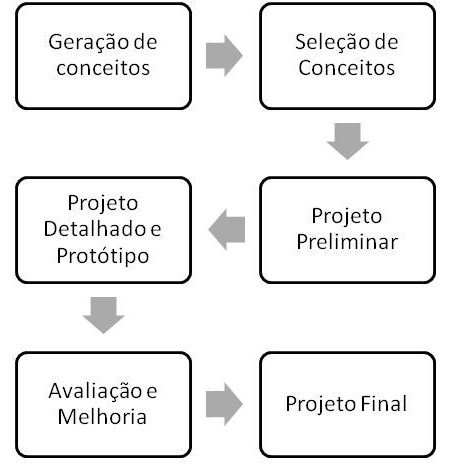
\includegraphics[scale=0.3]{editaveis/figuras/metodologia_de_desenvolvimento}
  \label{Metodologia de desenvolvimento}
  \caption{Metodologia de desenvolvimento}
  \end{center}
  \end{figure}
  \FloatBarrier
  
  A descrição de todas as etapas acima é relatada a seguir.
  
  \begin{enumerate}
   \parindent=1.25cm
   
   \item Geração de Conceito\\
      
      \noindent
      Divide-se em três:
      
      \noindent
      \subitem \textbf{Geração de ideias}
      
      Foi proposto ao grupo o desenvolvimento de um projeto preliminar de uma planta de abastecimento de água potável a partir 
      da umidade do ar. O projeto a ser realizado deveria ser inovador, de utilidade para seus consumidores finais, viável e
      que utilizasse fontes alternativas de energia para a solução do problema a ser idealizado pelo grupo.
      
      O método utilizado nesta etapa do projeto consiste em produzir reuniões onde todo o grupo estará presente, tais componentes 
      devem fornecer ideias que possam ser debatidas e analisadas por todos, sem descriminação.
      
      \noindent
      \subitem \textbf{Análise de tecnologia}
      
      Nesta fase devem ser realizadas vigorosas pesquisas externas a fim de investigar a existência de tecnologias que realizam o
      trabalho proposto ou que realizam processos similares. 
	    
      A proposta desta etapa é investigar os prós e contras das várias tecnologias pesquisadas e a viabilidade da tecnologia 
      a ser adotada.
      
      \noindent
      \subitem \textbf{Especificação de localização}
      
      Análise de requisitos sobre localização e avaliação das características do problema, a fim de identificar os possíveis 
      consumidores e sua localidade. 
      
      Os potenciais consumidores deste projeto são as famílias nordestinas, que tem suas vidas diariamente sendo ameaçadas 
      devido à falta de reserva de água.
   
  \item Seleção de Conceitos
  
    Esta etapa é responsável por avaliar quais conceitos gerados na fase anterior são relevantes e pela construção do
    embasamento teórico sobre os elementos determinados na etapa anterior. 
  
  \item Projeto Preliminar
  
    Esta etapa busca especificar o serviço e o produto com todos os seus componentes e processos necessários ao funcionamento.
    
    Esta fase é uma das mais importantes de todo o projeto, pois são tomadas decisões que serão o suporte de todo o
    desenvolvimento deste. No projeto preliminar deste projeto foram estabelecidas as seguintes informações principais: 
    
    \begin{itemize}
     \item A região de implementação do projeto será no Município de Acari, situado mais especificamente na região do Seridó, 
	na Mesorregião Central Potiguar, no estado do Rio Grande do Norte, no Brasil.
     
     \item A tecnologia adotada será uma turbina eólica capaz de transformar a umidade do ar em água.
     
     \item Serão adotados critérios quanto a qualidade da água, eficiência da turbina e 
	monitoramento de todo o sistema de captação, armazenamento e distribuição.     
    \end{itemize}
    
  \item Projeto Detalhado e Protótipo
  
    O projeto detalhado se diferencia do projeto preliminar devido às alterações e correções implementadas.
    
    O protótipo do projeto será feito na plataforma de desenho Catia v5\_R19, este processo de construção deve ter como 
    base o projeto detalhado e as dimensões reais do produto, para ser feito em menor escala.

  \item Avaliação e Melhoria
  
    Antes do término do projeto e lançamento do serviço, algumas modificações devem ser feitas em busca de melhorias. 
    Dentre as técnicas utilizadas neste processo, serão recomendadas o Desdobramento da Função Qualidade
    (ou QFD, Quality Function Deployment) e da Análise de Valor.
    
    O Desdobramento da Função Qualidade (QFD) tem como foco principal às necessidades dos clientes, oferecendo as
    alternativas capazes de satisfazê-los. Ou seja, dentro da matriz QFD os requisitos do consumidor (o quê) relacionam-se
    com as características do serviço (como), para que possamos prover mudanças que aumentem a satisfação do cliente.
    
    A Análise de Valor tem como objetivo aumentar o valor relativo de cada componente do serviço prestado, o que pode 
    ser feito através da redução de custos ou através do aumento do nível do serviço. Deve-se, em uma primeira etapa,
    distinguir as funções básicas das secundárias, para em seguida identificar tudo o que possa oferecer diminuição de custos,
    principalmente em funções secundárias; e aumento do valor, em funções básicas.
    
  \item Projeto Final
  
    O projeto final deve conter as alterações propostas por meio das técnicas de avaliação e melhoria, em modelo semelhante
    ao do projeto preliminar, porém de forma extremamente mais completa.
    
  \end{enumerate}

  
  \section{Referencial Teórico}
  
    Essa seção aborda alguns conceitos chave referentes ao trabalho.
    
    \subsection{Sistema de captação da umidade do ar}
    
      \documentclass[12pt,openright,oneside,a4paper,brazil]{abntex2}
\usepackage[utf8]{inputenc}
\counterwithout{section}{section}
\counterwithout{figure}{chapter}
\counterwithout{table}{chapter}
\setlength{\parindent}{1.3cm}
\usepackage{indentfirst}
\setlength{\parskip}{0.2cm}
\usepackage[bottom=2cm,top=3cm,left=3cm,right=2cm]{geometry}
\usepackage{graphicx}
\graphicspath{{figuras/}}
\usepackage{placeins}
\usepackage{cite}
\usepackage{url}
\usepackage{breakurl}
\include{bibliografia}

\makeatletter
\setlength{\@fptop}{0pt}
\makeatother

\begin{document}

\textual
\begin{center}
 {\large Captação de água e materiais estruturais}\\[0.2cm]
 \end{center}
 
Dentre as inspirações de tecnologia a serem aplicadas no projeto, as que se destacaram foram a Eolewater, Maxwater, Skywater e Warkawater. As três primeiras se baseiam no cooling compression, porém com custos diferentes. A Quarta tem custo  extremamente baixo se comparado com as outras Três tecnologias, por causa da simplicidade dos materiais que a constituem.Contudo, produz valores significantemente menores de água, além de não gerar energia para os processos de controle da qualidade da água. Por não gerar energia, também descartamos o Skywater.

As duas primeiras se baseiam em turbinas eólicas autossuficientes que retiram a umidade do ar, condensam, purificam e distribuem. Devido a geometria dos rotores do Max water que não é tão eficiente como os rotores tradicionais, de turbinas eólicas comuns, foi escolhido como base O sistema da Eolewater, que está descrito na figura 2.

\begin{figure}[!ht]
\centering
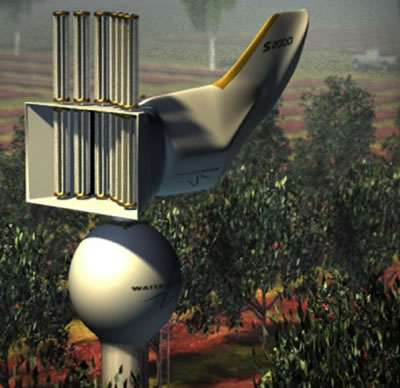
\includegraphics[scale=0.6]{max_water}
\caption[Caption title in LOF]{Max Water. Note como seus rotores são paralelos e verticais, tal configuração é ineficiente do ponto de vista aerodinâmico por gerar turbulência sobre os rotores vizinhos e gerar torques contrários com uma mesma direção de fluxo de ar.\footnotemark}

\label{Max_Water}
\end{figure}
\footnotetext{Disponível em: http://peswiki.com/index.php/Image:Max-water.jpg}

\begin{figure}[!htbp]
\centering
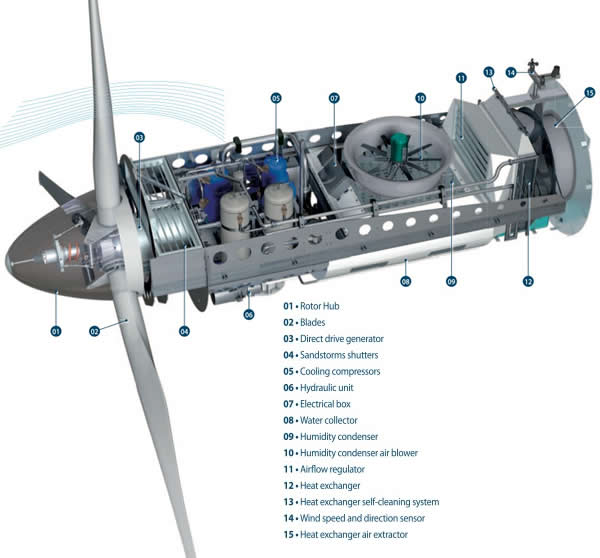
\includegraphics[scale=0.6]{Componentes}
\caption[Caption title in LOF]{Componentes de uma turbina Eolewater.\footnotemark}
\FloatBarrier
\label{Max_Water}
\end{figure}

\footnotetext{Fonte: RENEWABLE ENERGY DEVELOPMENT, 2012 }

As componentes de uma turbina eólica pouco mudam para essa acima,pois a Eolewater além de gerar energia para seu próprio funcionamento gera água, enquanto que a turbina eólica gera apenas energia.Na maioria das tecnologias de sucesso que pesquisamos, A Obtenção de água é feita pela condensação  a frio (cooling condensation), que é feita com o contato de ar com uma superfície fria. Para gerar essa superfície fria, um compressor comprime um fluido refrigerante, elevando sua temperatura. Esse fluido em alta temperatura passa por um trocador de calor e depois é expandido, o que causa uma queda ainda maior na temperatura do fluido. O fluido sob baixa temperatura circula por um condensador, por onde passa o ar atmosférico coletado. Esse condensador faz com que a temperatura do ar caia até o ponto de orvalho, temperatura na qual a água presente no ar se condensa em pequenas gotículas devido a saturação da quantidade de água no ar. A água proveniente da condensação é coletada e passa por tratamentos em UV e carvão ativado para que seja descontaminada e esteja pronta para consumo.



No Momento, o levantamento de materiais será apenas estrutural e se baseará em uma turbina eólica.

\begin{figure}[!htbp]
\centering
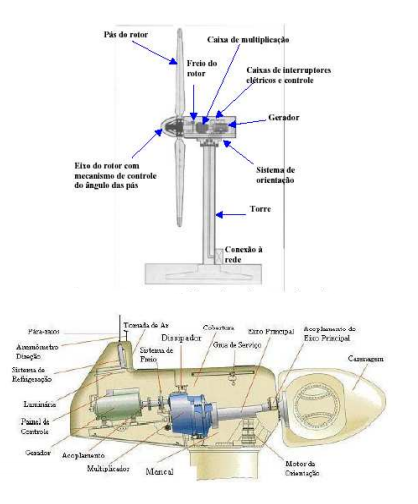
\includegraphics[scale=0.80]{turbina}
\caption[Caption title in LOF]{Seção de uma turbina eólica típica conectada à rede.\footnotemark}
\FloatBarrier
\label{Max_Water}
\end{figure}
\footnotetext{Fonte: USP, 2005 }

Dentro da turbina eólica temos os seguintes subconjuntos: torre, rotor, nacele, caixa de multiplicação (transmissão), gerador, mecanismos de controle, anemômetro, pás de rotor, biruta (sensor de direção). A torre é o elemento que sustenta o rotor e a nacele na altura adequada para o funcionamento da turbina eólica. Esse item é de elevada contribuição no custo inicial do sistema. O rotor é a componente onde as pás são conectadas e que realiza a transformação de energia cinética dos ventos em energia mecânica de rotação (ROSSI; OLIVEIRA; ALÉ, 2015).

	Nacele é um compartimento localizado no alto da torre que abrigam mecanismos do gerador (freios, caixa multiplicadora, embreagens, sistemas hidráulico, etc). Usaremos a Nacele para também abrigar os mecanismos de obtenção de água. 
	
	Caixa multiplicadora (transmissão) é o mecanismo que transmite a energia mecânica do eixo do rotar ao eixo do gerador. Gerador é o converterá energia mecânica do eixo em energia elétrica. Mecanismos de controle são os que supervisionam a velocidade média nominal que ocorre com maior frequência durante um determinado período. Anemômetro tem a função de medir a intensidade e a velocidade dos ventos. Pás do rotor captam o vento e converte sua potência ao centro do rotor. Biruta é um conjunto de sensores que captam a direção do vento (ROSSI; OLIVEIRA; ALÉ, 2015).
	
	Uma das componentes que se tem muito estudo é a pá rotativa. Ela pode ser feita com os seguintes materiais: madeira, aço, alumínio, fibra de vidro com resina poliéster, fibra de vidro com fibra de carbono, madeira com epóxi, fibra de carbono. A escolha do material vai depender da escolha do perfil aerodinâmico, que será estudado posteriormente. (PORTAL ENERGIA, 2015).
\begin{figure}[!htbp]
\centering
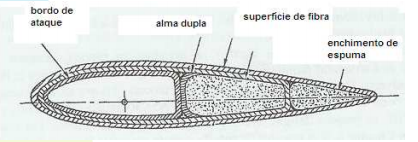
\includegraphics[scale=0.80]{pa}
\caption[Caption title in LOF]{Seção transversal de uma pá feita de fibra de vidro\footnotemark}
\FloatBarrier
\label{Max_Water}
\end{figure}
\footnotetext{Fonte: USP, 2005 }

Como pode ser visto as fibras são colocadas estruturalmente nas principais direções de propagação das tensões, quando em operação. A fibra de carbono e ou Kevlar são atualmente os compostos mais avançados que podem ser utilizados me áreas críticas (longarina da pá), mas tal material trem preços muito elevados (BARROS; VARELLA, 2015).  

Em relação ao suporte estrutural, ou torre, nas turbinas eólicas elas podem ser do tipo treliçadas, tubular e estaiada, no entanto, para a Eolewater as estruturas mais comuns são as duas últimas. As tores são constituídas de concreto e aço, tendo o peso em torno de 40 toneladas e 50 metros de comprimento (USP, 2005).

\begin{figure}[!htbp]
\centering
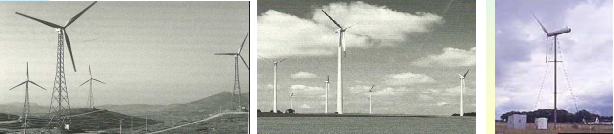
\includegraphics[scale=0.80]{torre}
\caption[Caption title in LOF]{Tipos de torre. Da esquerda para a direita: Treliçada, Tubular e Estaiada \footnotemark}
\FloatBarrier
\label{torre}
\end{figure}
\footnotetext{Fonte: USP, 2005 }

O modelo do dispositivo da Eolewater de gerar água por meio da energia eólica possui uma turbina WMS1000, de potência de30kW. O tempo de vida proposto para esse mecanismo é de 20 anos, dependendo das condições em que o motor é submetido ele pode gerar até 1200 litros de água por dia (mais informações na tabela abaixo). Como o dispositivo não necessita de quaisquer outros recursos para operar há um impacto mínimo sobre o meio em que é colocado (RENEWABLE ENERGY DEVELOPMENT, 2012).

\begin{figure}[!htbp]
\centering
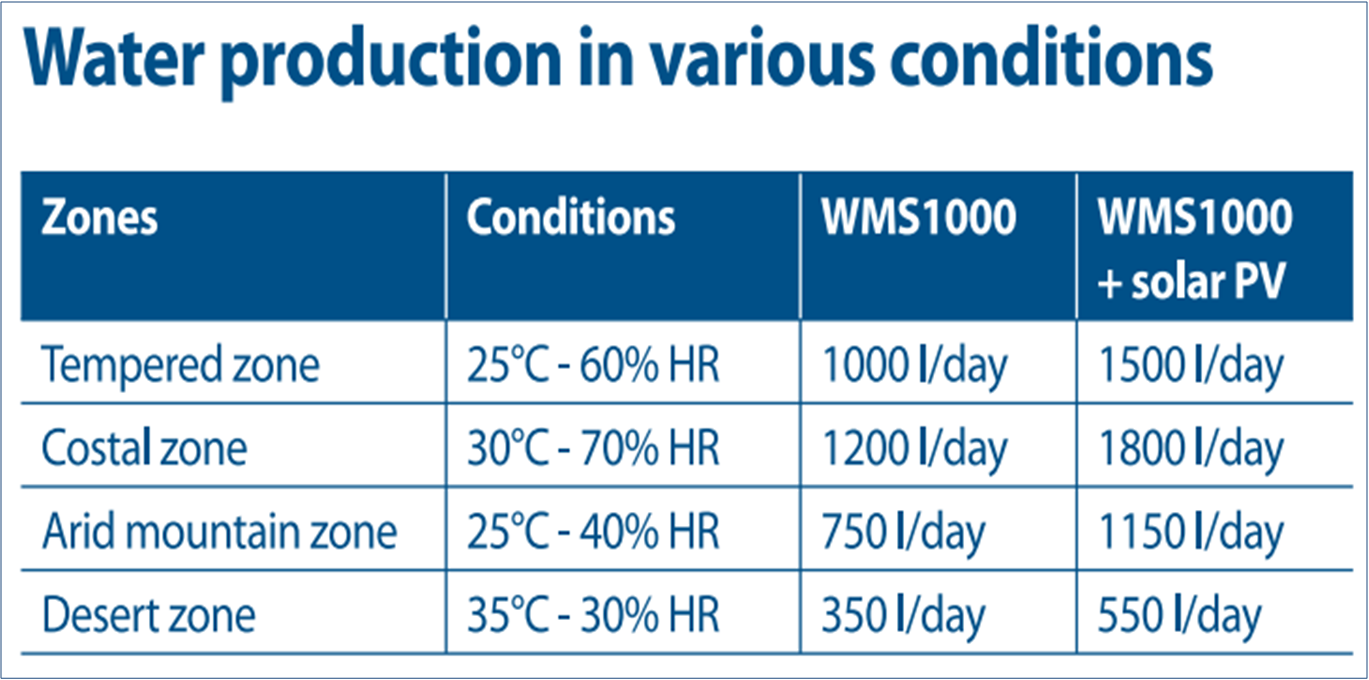
\includegraphics[scale=0.3]{condicoes}
\caption[Caption title in LOF]{Tabela de condições de umidade e temperatura para o rendimento de água \footnotemark}
\FloatBarrier
\label{condicoes}
\end{figure}
\footnotetext{Fonte: RENEWABLE ENERGY DEVELOPMENT, 2012}

Essa tecnologia possui um controle de pitch centrífuga para regular a velocidade do motor, tem um sistema de travagem rotor mecânica e elétrica, o qual evita danos nas lâminas giratórias (pás), ainda, contém um mastro de inclinação que integra a ação dos cilindros telescópicos com capacidade de empuxo de 115 toneladas. Deve-se destacar que os componentes que entram em contato com a água são feitos de uma liga de aço inoxidável especial que operará sem risco de corrosão (EOLE ÁGUA SAS, 2015).

	Uma tecnologia como essa segundo o site da Indústria Eólica uma turbina de vento abaixo de 100 kW vai custa por volta de US \$ 3.000 a US \$ 5.000  por quilowatt de capacidade. Portanto, levando em conta as especificações técnicas do Turbine WMS1000 abaixo a tecnologia é eficiente, mas cara (RENEWABLE ENERGY DEVELOPMENT, 2012).
	
\begin{figure}[!htbp]
\centering
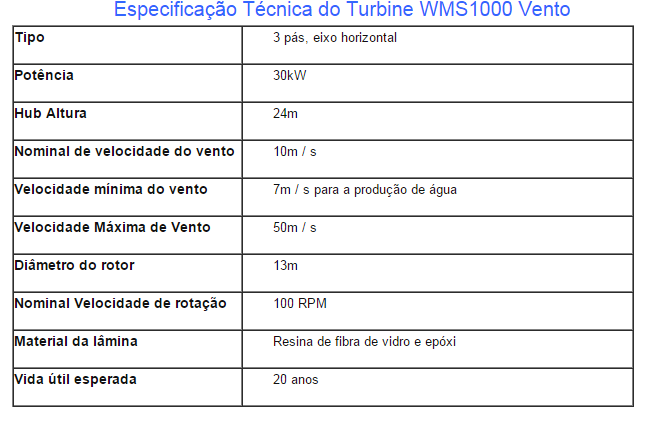
\includegraphics[scale=0.8]{especificacao}
\caption[Caption title in LOF]{Especificação Técnica do Turbine WMS1000 Vento \footnotemark}
\FloatBarrier
\label{Especificacoes}
\end{figure}
\footnotetext{Fonte: RENEWABLE ENERGY DEVELOPMENT, 2012}
 
A outra tecnologia, Warawater, por sua vez é uma tecnologia muito barata se comparada com a mencionada anterior. Essa custa cerca de US\$ 500 e pode ser construída em menos de uma semana com uma equipe de quatro pessoas e materiais existente localmente (DUARTE, 2015).

	Os materiais necessários para a sua construção de sua estrutura são: recipiente de coleta, bambu e um revestimento interno de plástico reciclado (rede). Sua torre possui em média 10 metros de altura, com 60 Kg e pode suprir até 100 litros de água por dia (TIMES, 2014).
\begin{figure}[!htbp]
\centering
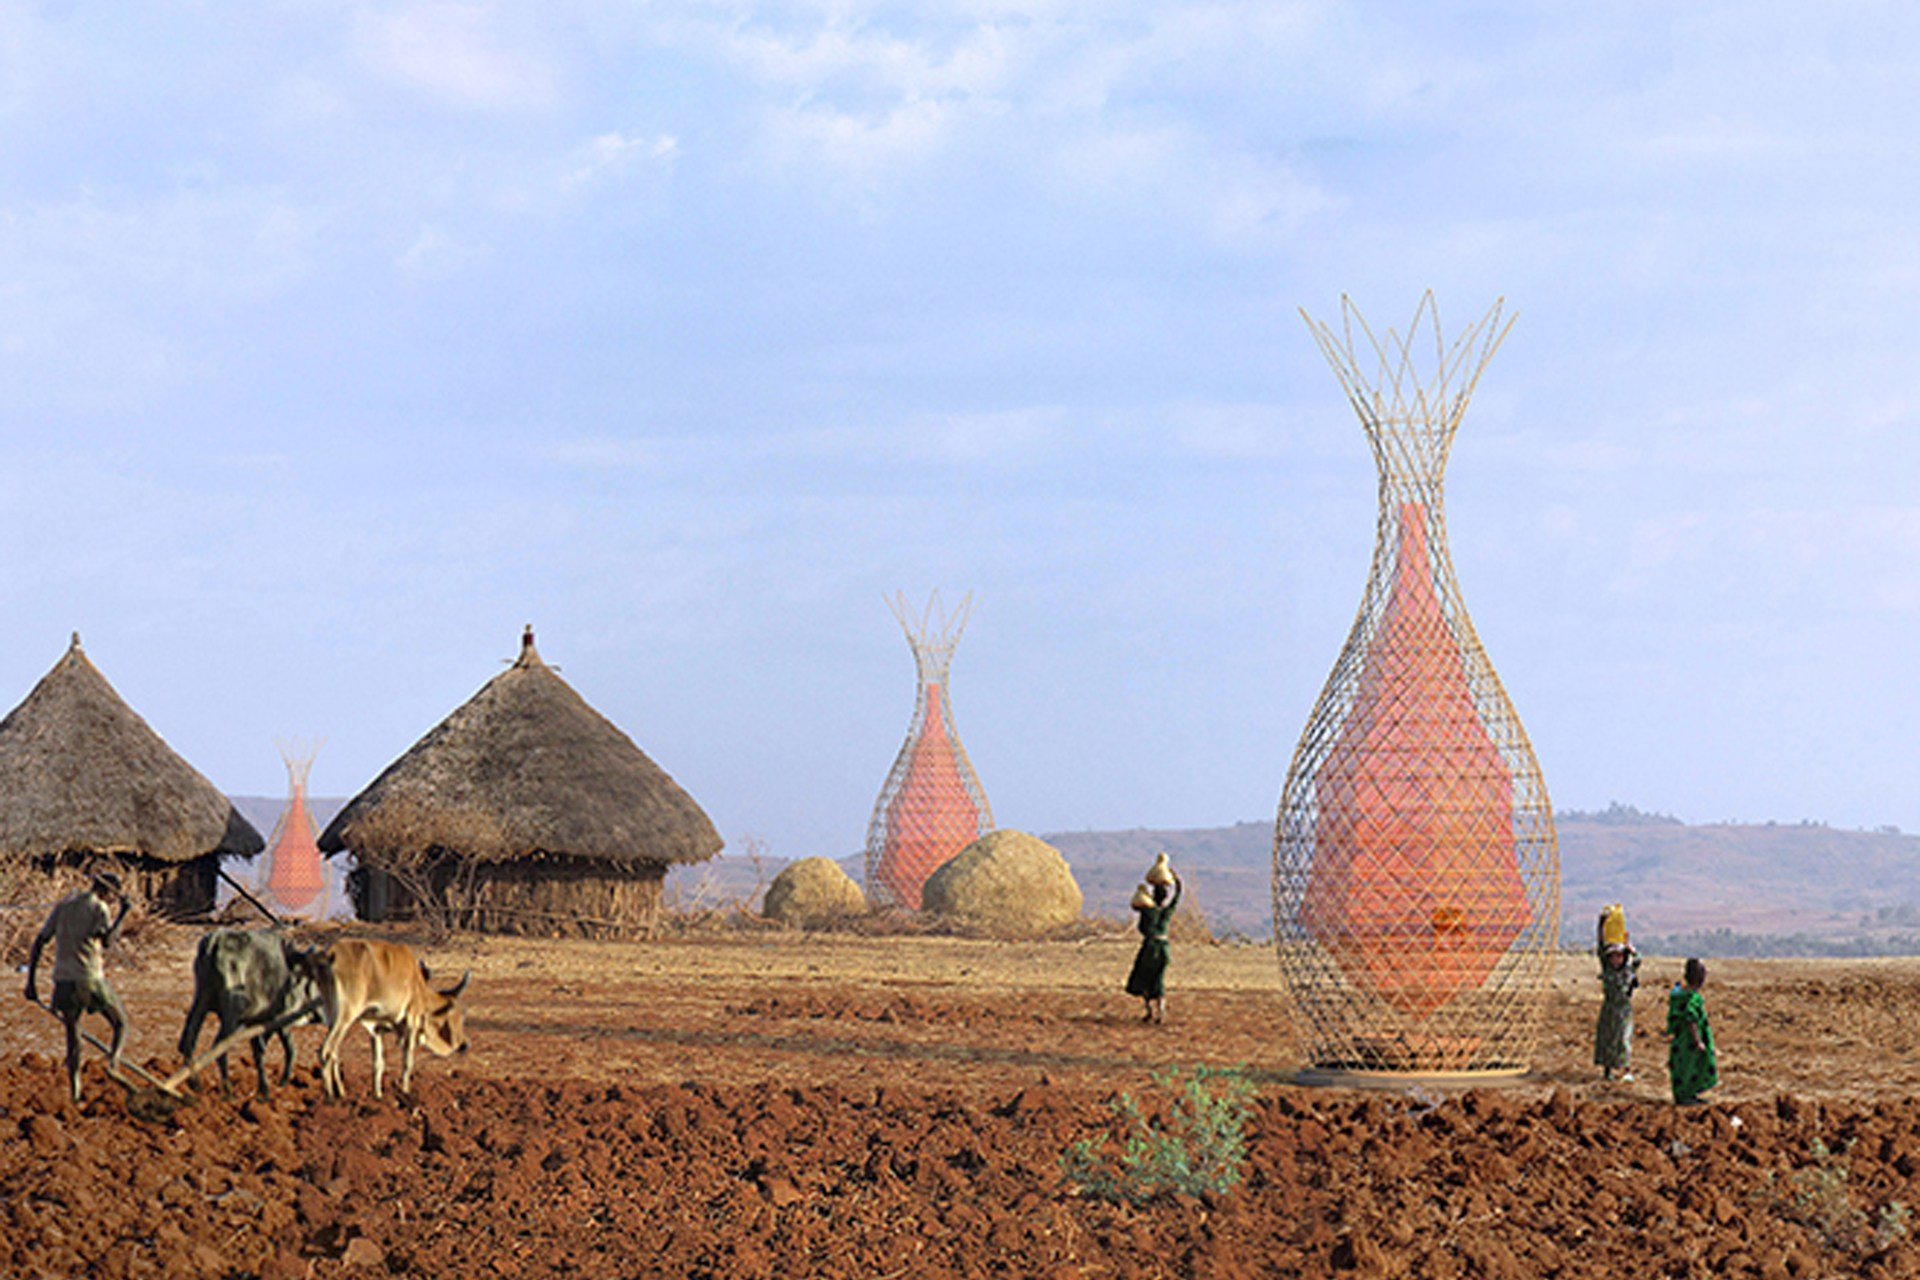
\includegraphics[scale=0.3]{warkawater}
\caption[Caption title in LOF]{Utilização da tecnologia warkawater por uma população carente  \footnotemark}
\FloatBarrier
\label{Especificacoes}
\end{figure}
\footnotetext{Fonte: DUARTE, 2015}

\bibliographystyle{abnt-alf}
\bibliography{bibliografia}

\end{document}
    
    \pagebreak
    \subsection{Matriz energética}
    
      Na contemporaneidade, quando se fala de geração de energia, em qualquer local do mundo a primeira questão a ser levantada
é a de maior distribuição possível juntamente com a maior viabilidade econômica envolvida. Estes foram dois parâmetros 
primordiais para se escolher a energia renovável para ser implantada dentro do projeto.

A Matriz Energética do Projeto foi divida em três áreas apresentadas a seguir.

  \subsubsection{Fontes Energéticas Referenciais}
    
    No decorrer do período de elaboração do escopo do projeto, várias possíveis soluções foram levantadas e, em seguida, 
    discutidas com o intuito de se chegar em um sistema que atendesse da melhor formar os requisitos iniciais do projeto.
    Dentre todas as opções disponíveis, foram pré-selecionadas três que, em princípio, se destacaram. São elas:
    
    \begin{itemize}
      \item \textbf{Eole Water}: uma turbina eólica autossuficiente que capta a água a partir de um sistema de refrigeração
	que faz com q a água no ar se condense ao entrar em contato com suas pás.
     
      \item \textbf{Maxwater}: um moinho de vento vertical, com um sistema muito semelhante ao primeiro, mas que possui custo,
	produção diferenciados.
      
      \item \textbf{Warkawater}:torre feita de bambu e que é forrada por dentro com uma malha plástica, que retém gotículas
	de orvalho. Esse sistema é passivo e não necessita de energia para produção de água já que funciona de forma passiva.
    \end{itemize}
  
    Dois requisitos muitos importantes para a escolha do sistema foram a necessidade do uso de uma fonte energética renovável
    e de que a água fosse analisada em tempo real. Observando o segundo requisito se percebe que existe a necessidade da
    implementação de sensores e de um sistema que envie todos os dados recolhidos por tais sensores. Nesse contexto pensou-se 
    primeiramente no uso de painéis solares fotovoltáicos, em um segundo momento, levando em consideração a região propícia à 
    implementação de um parque eólico e escolha do sistema Eolewater, decidiu-se por utilizar o excedente de energia gerado 
    pela turbina eólica para suprir as necessidades dos sistemas embarcados.
  
    A premissa do uso do potencial dos ventos para geração de trabalho data de milhares de anos atrás, onde essas tecnologias
    eram usadas principalmente para o bombeamento de água e para moagem de grãos. As primeiras tentativas do uso da energia
    eólica para geração de eletricidade foram no século XIX, ma só na década de 1970 é que essa tecnologia foi aplicada em
    escala comercial.
    
    A avaliação do potencial eólico de uma região requer trabalhos sistemáticos de coleta e análise de dados sobre a velocidade
    e o regime de ventos. Geralmente, uma avaliação rigorosa requer levantamentos específicos, mas dados coletados em 
    aeroportos, estações meteorológicas e outras aplicações similares podem fornecer uma primeira estimativa do potencial
    bruto ou teórico de aproveitamento da energia eólica.
    
    Embora ainda haja divergências entre especialistas e instituições na estimativa do potencial eólico brasileiro, 
    vários estudos indicam valores extremamente consideráveis. Até poucos anos, as estimativas eram da ordem de 20.000 MW.
    Hoje a maioria dos estudos indica valores maiores que 60.000 MW.
    
    As primeiras turbinas eólicas de uso comercial tinham a capacidade de produção elétrica entre 10kW e 50kW, já
    as máquinas de grande porte atuais tem uma potência superior a 1Mw. 
    
  \subsubsection{Técnicas e métodos de conversão e armazenamento}
    
    Um dos desafios do projeto foi estabelecer a demanda de água para a região selecionada e a partir disso dimensionar a
    estrutura física necessária de acordo com os requisitos. Dentre os modelos analisados pela equipe, a turbina de vento 
    mais favorável foi a Eolewater, modelo WMS100 Wind Turbine da empresa EoleWater, uma turbina de eixo horizontal que
    apresenta resultados satisfatórios à proposta e servirá de base de estudo para a implementação do projeto na área 
    energética.
    
    Apesar dos avanços nessa área, a energia eólica não possui uma capacidade de produção muito grande, por isso deve-se
    focar no requisito eficiência de conversão. Algumas formas de aperfeiçoar a produção estão relacionadas à dimensão do 
    gerador, aerodinâmica, materiais utilizados, projeção da estrutura e logística.
    
    Partindo dessa necessidade, o gerador exerce função primordial no funcionamento da turbina, pois é ele quem converte a
    energia mecânica em energia elétrica que alimenta todo o sistema. Dessa forma, temos o seguinte esquema de funcionamento:
    Os ventos fazem com que as pás do rotor girem, consequentemente girando o rotor. Este, por sua vez, converte a energia 
    cinética dos ventos em energia mecânica de rotação. Esse conjunto conectado a um eixo transmite essa rotação para o
    gerador. O gerador finalmente converte a energia mecânica em energia elétrica que alimenta todos os outros componentes
    eletrônicos (controle) e mecânicos da turbina.
    
    A produção de energia elétrica estimada da turbina é de aproximadamente 30kW (a produção real depende do diâmetro do rotor,
    rendimento do sistema, velocidade dos ventos, condições climáticas da região). Essa energia produzida alimentará os
    componentes da turbina e a energia remanescente será utilizada pela estação de controle e armazenada em baterias para
    que seja utilizada em situações emergenciais.
    
    Dessa forma, temos a seguinte distribuição energética:
    
    \begin{figure}[!ht]
    \centering
    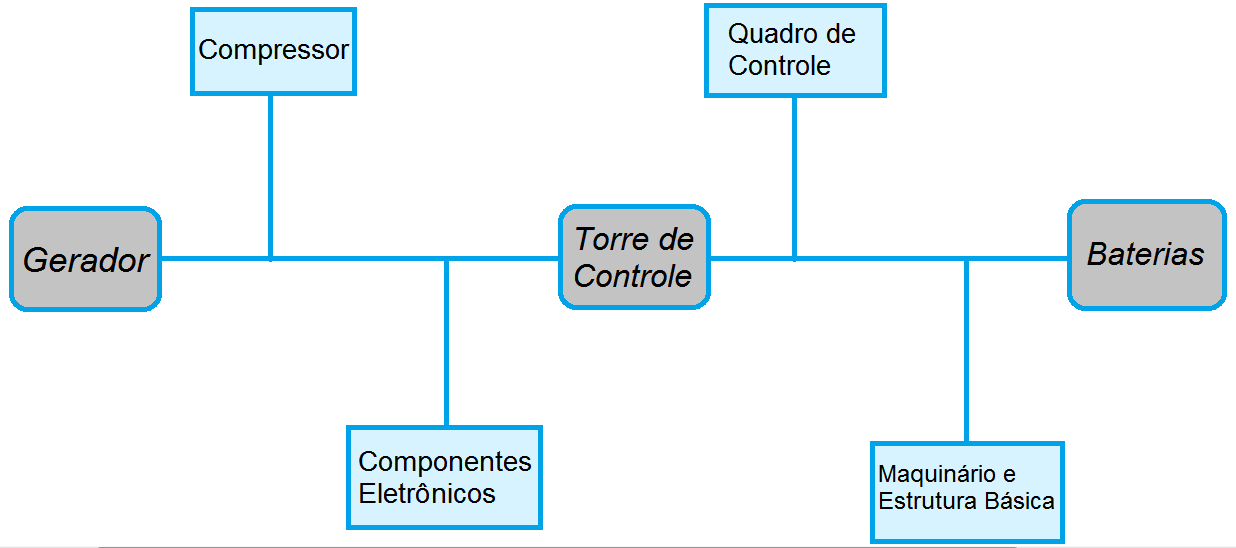
\includegraphics[scale=0.45]{editaveis/figuras/distribuicao_energetica}
    \caption{Distribuição energética}
    \label{distribuicao_energetica}
    \end{figure}
    
    \begin{enumerate}
     \item Geração de eletricidade (aproximadamente 30kW);
     \item Alimentação do compressor e componentes eletrônicos da turbina;
     \item Direcionamento a torre de controle;
     \item Distribuição no quadro de controle;
     \item Alimentação elétrica do maquinário e estrutura básica;
     \item Direcionamento de energia remanescente para as baterias emergenciais.
    \end{enumerate}
    
  \subsubsection{Eficiência Energética}
  
    A turbina eólica, ou aerogerador, é uma máquina capaz de absorver a potência cinética do vento por meio de um rotor
    aerodinâmico, convertendo este movimento em potência mecânica de eixo (torque vs rotação),  que é transformada em
    potência elétrica (tensão \textit{vs} corrente) por intermédio de um gerador elétrico.
    
    A parte estrutural de geração de energia de uma turbina é constituída por um rotor e pela torre que a sustenta,
    pela transmissão/multiplicação e pelo conversor. Ela somente consegue extrair energia através da energia cinética do 
    ar que passa pelo interior da área interceptada pelas pás rotativas.  
    
    Energia eólica provém da radiação solar. Se considerarmos que, aproximadamente, 2\% da energia solar que a Terra absorve,
    é convertida em energia cinética dos ventos, teremos uma estimativa da energia total disponível dos ventos ao redor
    do planeta.
    
    Os ventos (massas de ar em movimento),são influenciados por diferentes aspectos dentre os quais se destacam a rugosidade
    do solo, os obstáculos e o relevo da região, e possuem energia cinética que pode ser aproveitada com o uso de aerogeradores.
    
    Dessa forma, a energia cinética $E_C$, contida em uma amostra de volume de ar, $A$ x $\delta x$, com densidade do ar $\rho$, 
    movendo-se com uma velocidade, $v$,  onde $A$ é uma unidade de área perpendicular à direção dos ventos e $\delta x$ é paralelo 
    à direção dos  ventos, é dada por:
    
    $$ E_C = \frac{Mv^2}{2} = \frac{\rho A {\delta x} v^2}{2} $$
    
    A primeira vista, imagina-se que a máxima energia retirada dos ventos por uma turbina eólica é a energia cinética dos
    ventos que atravessam um círculo formado pela área das pás. Contudo, o próprio vento possui energia cinética na esteira
    do rotor, fazendo com que nem toda energia seja retirada. Segundo uma teoria criada por Betz* (para um modelo ideal), 
    a eficiência aerodinâmica do rotos estaria limitada a 59,3\% da energia presente nos ventos.
    
    O rotor é o primeiro estágio de conversão da energia do vento em eletricidade. Os estágios seguintes são a transmissão
    e o próprio gerador, que adéqua às velocidades de rotação e converte a energia mecânica em energia elétrica, 
    respectivamente.
    
    Em média, a eficiência de conversão dos modernos aerogeradores está dividida como ilustra a Figura ~\ref{eficiencia_conversao_aerogeradores}.
    
    \begin{figure}[!ht]
    \centering
    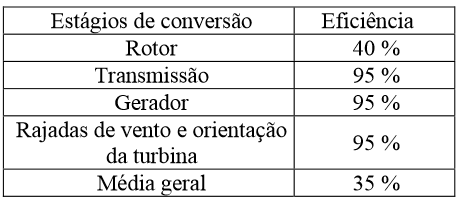
\includegraphics[scale=0.7]{editaveis/figuras/eficiencia_conversao_aerogeradores}
    \caption{Eficiência de conversão dos aerogeradores modernos}
    \label{eficiencia_conversao_aerogeradores}
    \end{figure}
    
    Na contemporaneidade, os parâmetros de rotores utilizados nos aerogeradores modernos são de duas ou três pás.
    Isso graças à relação de potência extraída por área de varredura do rotor (muito superior ao rotor multipás) para 
    velocidades mais elevadas. Tais características são aceitáveis em sistemas de geração de eletricidade, porém se tornam
    inviáveis em sistemas que requeiram altos momentos de força e/ou carga variável.
    
    Rotores modernos, com mais de três pás, são usados somente quando há necessidade de um grande torque de partida, ou seja, 
    basicamente, bombeamento mecânico de água. Aerodinamicamente, no entanto, grande número de pás e alto torque de partida,
    diminuem a eficiência do sistema. 

    Sendo assim, o desenvolvimento de pás para aerogeradores deve ser resultante da integração entre estes fatores.
    Com o estágio atual da tecnologia, a dificuldade de fabricação não reside na aerodinâmica, mas sim na construção
    e resistência dos materiais que compõem as pás, que devem responder a diferentes exigências da máquina eólica,
    além de ser necessário que sejam resistentes, rígidos, leves e de baixo custo.
    
    As perdas de transmissão relacionam-se diretamente ao atrito que existe entre as engrenagens.
    Em velocidades de giro fixas, as perdas variam pouco, podendo-se assumir que são uma porcentagem fixa
    da potência nominal. Esta porcentagem real depende da qualidade da transmissão, mas um valor razoável
    pode ser em torno de 2\% da potência em cada etapa de engrenamento. Como a transmissão consome certa quantidade de
    energia, as perdas podem ser consideráveis em baixas potências, já que o rendimento nestes casos é menor.
    
    Para que a geração de eletricidade a partir do movimento do ar seja plausível, técnica e economicamente, alguns fatores
    ganham relevância. A velocidade dos ventos é o fator mais crítico na determinação da energia que será obtida de um
    aerogerador, e também seu custo. Outros fatores seriam:
    \begin{itemize}
     \item \textbf{Topografia}: o ar é mais frio durante a noite e tende a ocupar regiões próximas ao solo, além de produzir
	pouca quantidade de vento. Por isso devem ser escolhidas áreas mais elevadas. Para a escolha dessas áreas devem ser
	observadas também: facilidade de locomoção até a instalação, proximidade ao ponto de consumo, espaço necessário
	para manutenções e evitar áreas muito frias, a fim de não danificar o aerogerador.
	
     \item \textbf{Barreiras Naturais}: prédios, árvores, plantações e construções elevadas que podem diminuir
	a velocidade do vento e turbulência, danificando o equipamento.
      
     \item \textbf{Superfície}: quanto mais acidentado o terreno (maior rugosidade), com plantações, construções, árvores, entre outros,
	mais alta a torre deve ser.
      
     \textit{Obs.:} Quando não especificada a altura na qual ocorreu a medição da velocidade dos ventos,
	consideramos a altura padrão internacional de 10 metros acima do solo, ou a altura em que cada gerador está operando. 
     
    \end{itemize}
    
    \pagebreak
    \subsection{Sistema eletrônico de monitoramento e controle da qualidade da água}
      
      \subsubsection{Parâmetros de qualidade da água}
        
        A poluição e uso irracional e inadequado da água comprometem a disponibilidade de água em padrões de qualidade apropriados 
ao uso da geração atual e das que estão por vir. Dessa maneira, faz-se necessário o monitoramento das águas que serão
destinadas ao abastecimento da população.

Os indicadores ambientais surgiram a partir da crescente preocupação socioambiental referente ao desenvolvimento.
Os indicadores tornaram-se fundamentais no processo decisório das políticas públicas e no acompanhamento de seus efeitos.
Esta dupla vertente apresenta-se como um desafio permanente de gerar indicadores e índices que tratem um número cada vez 
maior de informações, de forma sistemática e acessível, para os tomadores de decisão \cite{cetesbIndiceQualidadeH2O}.

Existe um indicador chamado Índice de Qualidade das Águas (IQA), o qual foi desenvolvido pela 
Companhia de Tecnologia de Saneamento Ambiental do Estado de São Paulo (CETESB) por meio da consulta à especialistas 
em qualidade da água, os quais apontaram parâmetros a serem avaliados acompanhados de seus respectivos pesos e a 
condição com que se apresenta cada parâmetro, de acordo com uma lista de valores. Desses parâmetros, os 9 (nove) 
principais foram selecionados. Para esses, foram estabelecidas curvas de variação de qualidade das águas de acordo 
com o estado ou a condição de cada parâmetro. Essas curvas são apresentadas na Figura ~\ref{graficos_parametros}.

A maior parte dos parâmetros levados em consideração no cálculo do IQA são indicadores de contaminação propiciada
pela emissão de esgotos domésticos.

O IQA é o principal índice de qualidade da água utilizado em todo o país. A finalidade de tal índice é transformar 
diversos dados relacionados à qualidade da água em um único número, que representa o nível de qualidade da água.

De acordo com a Agência Nacional de Águas \cite{anaGovIndicadores}, como desvantagens do uso do IQA, deve-se citar o fato de
o índice não contemplar vários parâmetros importantes para o abastecimento público, tais como:

\begin{itemize}
 \item Substâncias tóxicas (ex: metais pesados, pesticidas, compostos orgânicos);
 \item Protozoários patogênicos;
 \item Substâncias que interferem nas propriedades organolépticas da água.
\end{itemize}

Os nove parâmetros com seus respectivos pesos são apresentados a seguir:

\begin{figure}[!h]
\centering
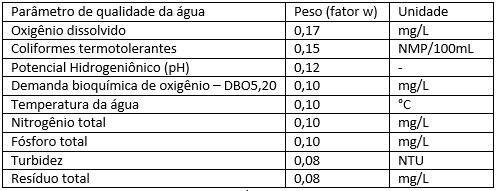
\includegraphics[scale=0.8]{editaveis/figuras/tabela_parametros_unidade}
\FloatBarrier
\label{tabela_parametros_unidade}
\caption[Parâmetros de qualidade da água do índice IQA e seus respectivos pesos]
  {Parâmetros de qualidade da água do índice IQA e seus respectivos pesos. \footnotemark}
\end{figure}
\footnotetext{Fonte: \cite{anaGovIndicadores}; \cite{cetesbIndiceQualidadeH2O}}

Além de seu peso ($w$), cada parâmetro possui um valor de qualidade ($q$), o qual é obtido do respectivo gráfico de qualidade
em função de sua concentração ou medida. Observe a figura abaixo:

\begin{figure}[!h]
\centering
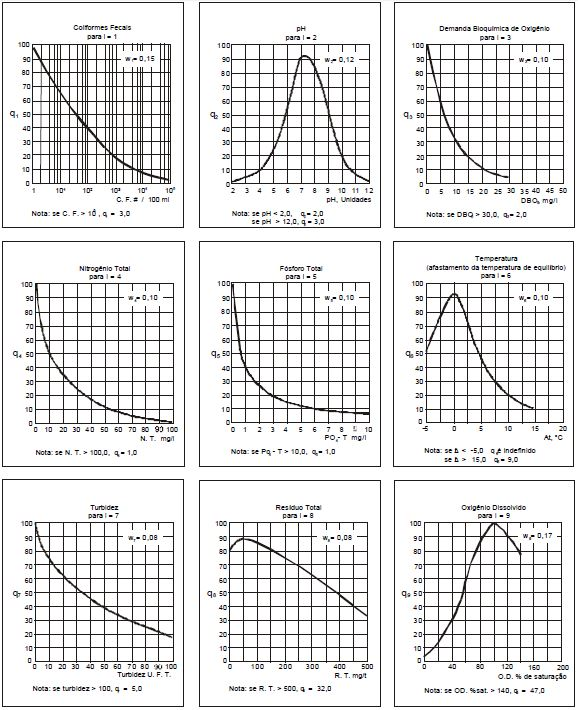
\includegraphics[scale=0.5]{editaveis/figuras/graficos_parametros}
\label{graficos_parametros}
\caption[Curvas de variação de qualidade das águas]{Curvas de variação de qualidade das águas.\footnotemark}
\end{figure}
\FloatBarrier
\footnotetext{Fonte: \cite{cetesbIndiceQualidadeH2O}}

O cálculo do IQA é dado da seguinte forma:

$$ IQA = \prod_{i = 0}^{n} {q_i}^{w_i} $$

\begin{center}
Fonte: \cite{anaGovIndicadores}
\end{center}

Onde:

\begin{itemize}
 \item $IQA$: Índice de Qualidade das Águas, representado por um número de 0 a 100;
 \item $q_i$: qualidade do i-ésimo parâmetro, representado por um número entre 0 e 100, obtido do respectivo gráfico de qualidade, em função de sua concentração ou medida;
 \item $w_i$: peso correspondente ao i-ésimo parâmetro fixado em função da sua importância para a conformação global da qualidade, isto é,  um número de 0 a 1, de forma que:
 
    $$ \sum_{i=1}^n w_i = 1 $$
    Sendo $n$ o número de parâmetros que entram no cálculo do IQA.
\end{itemize}

A tabela a seguir apresenta a classificação da água de acordo com o valor do IQA:

\begin{figure}[!h]
\centering
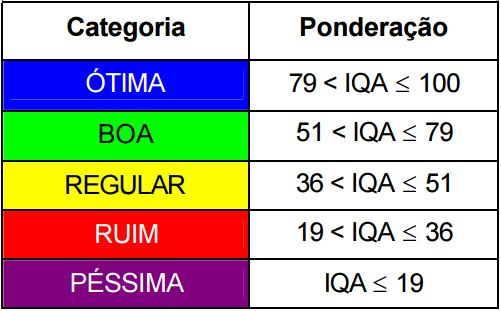
\includegraphics[scale=0.7]{editaveis/figuras/tabela_classificacao_IQA}
\label{tabela_classificacao_IQA}
\caption[Classificação da água de acordo com o IQA]{Classificação da água de acordo com o IQA.\footnotemark}
\end{figure}
\FloatBarrier
\footnotetext{Fonte: \cite{cetesbIndiceQualidadeH2O}}

Segundo a \cite{anaGovIndicadores}, a descrição dos parâmetros que compõe o IQA pode ser efetuada da seguinte maneira:

\begin{itemize}
 \item \textbf{Oxigênio dissolvido (OD)}: é um fator limitante para a manutenção da vida aquática e de processos de 
    autodepuração em sistemas aquáticos naturais e estações de tratamento de esgotos \cite{cetesbOxigenioDissolvido}.
    Águas limpas têm concentração de oxigênio, na maioria das vezes, maior ou igual a 5 mg/L. No que se refere aos processos que
    contribuem para a introdução do oxigênio na água, pode-se citar, além da fotossíntese, determinados processos físicos 
    os quais dependem das características hidráulicas dos corpos d’água, por exemplo: velocidade da água.
    
 \item \textbf{Coliformes termotolerantes}: São bactérias não patogênicas que ocorrem no trato intestinal de animais de sangue
    quente e são indicadoras de poluição da água causada pelos esgotos domésticos. Quando há grande quantidade dessas bactérias
    na água, há possibilidade de existir microorganismos capazes de transmitir doenças de veiculação hídrica.
    
 \item \textbf{Potencial Hidrogeniônico (pH)}: O pH (medida que determina a acidez ou basicidade de uma mistura) é capaz de
    alterar o metabolismo de diversas espécies aquáticas. Dessa forma, o CONAMA estabelece que o pH deve estar entre 6 e 9 
    para a proteção da vida aquática. O pH também afeta a intensidade do efeito das substâncias tóxicas nos seres aquáticos,
    tais quais os metais pesados.
    
 \item \textbf{Demanda Bioquímica de Oxigênio (DBO5,20)}: representa a quantidade necessária de oxigênio para oxidar a matéria
    orgânica aquática por meio da decomposição microbiana aeróbia. A ocorrência de altos valores de DBO5,20 acarreta na diminuição
    dos valores de oxigênio dissolvido (OD). A sigla DBO5,20 equivale à quantidade de oxigênio consumido em 5 dias a uma temperatura de 20C.
    A causa de altos valores de DBO5,20 numa amostra d’água é geralmente devido à emissão de dejetos de origem orgânica,
    principalmente esgotos domésticos.
    
 \item \textbf{Temperatura da água}: influencia em diversos parâmetros físico-químicos da água (ex: tensão superficial e a
    viscosidade) além de afetar o crescimento e reprodução de espécies aquáticas.
    
 \item \textbf{Nitrogênio total}: O nitrogênio pode ocorrer nos corpos d’água em diversas formas (orgânica, amoniacal, nitrito 
    e nitrato). Os nitratos são tóxicos aos humanos.
    Além disso, como os compostos de nitrogênio nutrem os processos biológicos, a grande concentração de nitrogênio 
    (juntamente com outros nutrientes) em corpos d’água causa a eutrofização, que prejudica o abastecimento público e
    a preservação da vida aquática.
    A principal fonte de nitrogênio em corpos d’água é o lançamento de esgotos sanitários e efluentes industriais.
    Em áreas agrícolas, o escoamento da água das chuvas em solos que receberam fertilizantes também é uma fonte de nitrogênio,
    assim como a drenagem de águas pluviais em áreas urbanas.
    
 \item \textbf{Fósforo total}: Assim como o nitrogênio, o fósforo (em excesso) causa a eutrofização das águas.
    As principais fontes de fósforo são os esgotos domésticos, pelo fato de eles terem a presença de detergentes
    superfostadados e das próprias fezes. Além disso, a drenagem pluvial de áreas agrícolas e urbanas também é uma fonte 
    significativa. Entre os efluentes industriais destacam-se os das indústrias de fertilizantes, alimentícias, laticínios, 
    frigoríficos e abatedouros.
    
 \item \textbf{Turbidez}: indica o grau de atenuação que um feixe de luz sofre ao atravessar a água. Tal atenuação é devida à
    absorção e espalhamento de luz causada pelos sólidos em suspensão. 
    A principal fonte de turbidez é a erosão dos solos (chuvas trazem os corpos sólidos).
    Porém, além desta, é possível citar as atividades de mineração, bem como o lançamento de esgotos e de efluentes industriais,
    como causadoras da turbidez nas águas.
    
 \item \textbf{Resíduo total}: é a matéria a qual permanece após a evaporação, secagem ou calcinação da amostra de água durante um 
    determinado tempo e temperatura.    
\end{itemize}

Existe uma empresa chamada Clean Environment Brasil \cite{cleanEnvironmentBrasil}, que fornece equipamentos de monitoramento e controle da água à ANA 
(Agência Nacional de Águas). Eles produzem várias sondas multiparamétricas (conseguem monitorar vários parâmetros em uma sósonda).

Seria interessante utilizar a sonda YSI EXO, que coleta dados de 6 sensores substituíveis, pois ela também é usada pela ANA para determinar a qualidade da água.

As opções de sensores para esse tipo de sonda são:

\begin{itemize}
 \item Oxigênio dissolvido;
 \item Matéria Orgânica Dissolvida (fluorescência);
 \item pH ou pH/ORP;
 \item Profundidade (que já é integrado);
 \item Algas totais (canal duplo para clorofila e algas azuis/verdes);
 \item Turbidez.
\end{itemize}

Assim, com apenas um equipamento relativamente leve (3,6 kg com baterias e sensores instalados) de pequenas
dimensões (phi = 7,62cm e comprimento = 71,10cm) é possível monitorar a maioria dos parâmetros do índice IQA \cite{cleanEnvironmentBrasil}.







      
      \subsubsection{Revisão Legislativa de Saneamento e Distribuição de Água}
      	Considerando que nossa empresa deverá distribuir água com qualidade suficiente para consumo humano, baseamos no decreto nº7.217, de de 21 de junho de 2010, que regulamenta a lei nº 11.445, de 5 de janeiro de 2007, que estabelece diretrizes nacionais para o saneamento básico.

Art. 1º Esta portaria dispõe sobre os procedimentos de controle e de vigilância de qualidade da água para consumo humano e seu padrão de potabilidade.

Art. 2º Esta portaria se aplica à água destinada ao consumo humano proveniente, de sistema e solução alternativa de abastecimento de água.

Art. 3º Toda água destinada ao consumo humano distribuída coletivamente por meio de sistema ou solução alternativa coletiva de abastecimento de água, deve ser objeto de controle e vigilância de qualidade da água.

Art. 4º Toda água destinada ao consumo humano proveniente de solução alternativa individual de abastecimento de água independentemente da forma de acesso da população, está sujeita à vigilância de qualidade de água.

Art. 5º Para fins desta portaria, são adotadas as seguintes definições:

I - Água para consumo humano: água potável destinada à ingestão, preparação e produção de alimentos e à higiene pessoal, independentemente da sua origem.

II – Agua potável: água que atenda ao padrão de potabilidade estabelecido nesta Portaria e que não ofereça riscos à saúde.

III - Padrão de potabilidade: conjunto de valores permitidos como parâmetro da qualidade da água para consumo humano, conforme definido nesta Portaria.

IV - Padrão organoléptico: conjunto de parâmetros caracterizados por provocar estímulos sensoriais que afetam a aceitação para consumo humano, mas que não necessariamente implicam riscos à saúde.

V - Água tratada: água submetida a processos físicos, químicos ou combinação destes, visando atender ao padrão de potabilidade.

VI – Sistema de abastecimento de água para consumo humano: instalação composta por um conjunto de obras civis, materiais e equipamentos, desde a zona de captação até as ligações prediais, destinada à produção e ao fornecimento coletivo de água potável, por meio de rede de distribuição.

VII - Solução alternativa coletiva de abastecimento de água para consumo humano: modalidade de abastecimento coletivo destinada a fornecer água potável, com captação subterrânea ou superficial, com ou sem canalização e sem rede de distribuição.

VIII - Solução alternativa individual de abastecimento de água para consumo humano: modalidade de abastecimento de água para consumo humano que atenda a domicílios residenciais com uma única família, incluindo seus agregados familiares.

IX - Rede de distribuição: parte do sistema de abastecimento formada por tubulações e seus acessórios, destinados a distribuir água potável, até as ligações prediais.

X - Ligações prediais: conjunto de tubulações e peças especiais, situado entre a rede de distribuição de água e o cavalete, este incluído.

XI - Cavalete: kit formado por tubos e conexões destinados à instalação do hidrômetro para realização da ligação de água.

XII - Interrupção: situação na qual o serviço de abastecimento de água é interrompido temporariamente, de forma programada ou emergencial, em razão da necessidade de se efetuar reparos, modificações ou melhorias no respectivo sistema.

XIII - Intermitência: é a interrupção do serviço de abastecimento de água, sistemática ou não, que se repete ao longo de determinado período, com duração igual ou superior a seis horas em cada ocorrência.

XIV - Integridade do sistema de distribuição: condição de operação e manutenção do sistema de distribuição (reservatório e rede) de água potável em que a qualidade da água produzida pelos processos de tratamento seja preservada até as ligações prediais.

XV - Controle da qualidade da água para consumo humano: conjunto de atividades exercidas regularmente pelo responsável pelo sistema ou por solução alternativa coletiva de abastecimento de água, destinado a verificar se a água fornecida à população é potável, de forma a assegurar a manutenção desta condição.

XVI - Vigilância da qualidade da água para consumo humano: conjunto de ações adotadas regularmente pela autoridade de saúde pública para verificar o atendimento a esta Portaria, considerados os aspectos socioambientais e a realidade local, para avaliar se a água consumida pela população apresenta risco à saúde humana.

XVII - Garantia da qualidade: procedimento de controle da qualidade para monitorar a validade dos ensaios realizados.

XVIII - Recoleta: ação de coletar nova amostra de água para consumo humano no ponto de coleta que apresentou alteração em algum parâmetro analítico.

XIX - Passagem de fronteira terrestre: local para entrada ou saída internacional de viajantes, bagagens, cargas, contêineres, veículos rodoviários e encomendas postais.


        
      \subsubsection{Projeto eletrônico e de controle da planta}
        
        
\textbf{Sensores}

Ao se expor todos os parâmetros de qualidade da água, é necessário se ter o conhecimento dos sensores que farão a
obtenção dessas informações. A seguir, se encontram uma série de sensores que foram pesquisados a fim de se ter uma 
idéia geral de quais equipamentos poderão ser utilizados no projeto. 

Sensores são dispositivos eletroeletrônicos que tem a propriedade de transformar em sinal elétrico a transformação
de uma grandeza física que esta relacionada a uma ou mais propriedade do material de que é feito o sensor. Esses elementos
são capazes de monitorar a variação de uma grandeza física e transmitir esta informação a um sistema em que a indicação
seja inteligível para nós ou para o elemento de controle do sistema. Os sensores são compostos por elementos denominados
transdutores que convertem uma grandeza de entrada em uma grandeza elétrica, que pode ser processada por um circuito
elétrico ou eletrônico \cite{vinay00}.

Existem diversos tipos de sensores os que julgamos necessários para o controle do sistema de capitação de água pela rotação
da turbina. São os sensores de umidade relativa do ar, sensores de velocidade e direção do vento (anemômetro), sensores
de nível e fluxo de entrada e saída de água, sensores de oxigênio, sensores de condutividade, sensores de pH, sensores
de turbidez, sensores de nitrato/nitrogênio, entre outros.

  \begin{enumerate}
  
    \item \textbf{Sensor da umidade do ar e temperatura}
      
	Características:
	
	\begin{itemize}
	 \item Processamento digital de sinal
	 \item Umidade relativa e temperatura do ar em um único sensor
	 \item Alta acurácia de leitura e linearização
	 \item Sinais de saída condicionados
	 \item Excelente estabilidade de longo termo
	 \item Baixo tempo de resposta
	 \item 100\% intercambialidade
	\end{itemize}

	Construção:
	
	O invólucro do sensor e do circuito eletrônico é moldado em plástico injetado e estabilizado para U.V.
	O invólucro do circuito é selado, sendo à prova de respingos e poeira. Todas as conexões elétricas
	são feitas através de um conector selado na base do sensor. O sensor opera de 0 a 100\% umidade relativa.
	Os transdutores internos não sofrem danos mesmo com condensação. O circuito digital do sensor realiza a
	compensação de temperatura e a linearização do sinal de saída. O armazenamento dos dados de calibração do
	 sensor em memória interna não volátil fornece uma maior acurácia nas leituras.
	 
	 \begin{figure}[!htbp]
	  \centering
	  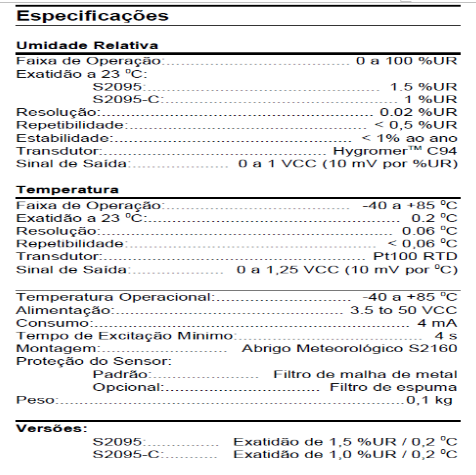
\includegraphics[scale=0.5]{editaveis/figuras/especificacao_sensor_umidade}
	  \caption[Especificação do sensor de umidade e temperatura]{Especificação do sensor de umidade e temperatura. \footnotemark}
	  \FloatBarrier
	  \label{especificacao_sensor_umidade}
	 \end{figure}
	 \footnotetext{Fonte: \cite{squitter}}
	 
    \item \textbf{Sensor de pH}
    
	O sensor de pH da água é de extrema importância para o projeto da “planta de abastecimento de água potável
	através da umidade do ar” pois monitora um dos índices de qualidade da água especificados pela \cite{anaGov}.
	
	\begin{center}
	 \textbf{Especificação do sensor de pH}
	\end{center}

	Para aplicações industriais, o método de medição de pH mais empregado é o eletrodo de vidro \cite{sole79}.
	Os eletrodos de pH possuem basicamente o mesmo funcionamento que as baterias: transferem uma tensão mínima que poderá
	ser detectada por um medidor ou um regulador de pH. A diferença é que os eletrodos de pH não produzem tensão de forma
	contínua, a não ser quando são introduzidos num líquido.
	
	\begin{center}
	 \textbf{Calibração de sensores de pH}
	\end{center}
	
	O período de calibração de um sensor de pH depende do contexto em que o sensor será aplicado e do tipo de sensor
	que será utilizado. O tipo de sensor a ser utilizado pode variar de acordo com parâmetros como temperatura.
	O sensor de pH pode vir acoplado a um sensor de condutividade, entre outros. Apesar de existirem vários tipos,
	todo eletrodo de pH requer calibração periódica. Uma calibração em dois pontos caracteriza um eletrodo com um
	medidor de pH específico. Uma desvantagem dos sensores de pH é que eles necessitam de calibração diária.
	Neste caso, seria necessário um funcionário que realizasse a calibração diariamente, ou de um sistema automatizado
	que realize a calibração.
	
	
    \item \textbf{Sensor ORP}
    
	O sensor ORP é similar ao sensor pH quanto ao seu funcionamento, porém, ao invés de seu eletrodo ser envolvido por
	vidro, é geralmente envolvido por platina ou ouro, devido ao fato de esses metais não interferirem nas reações químicas.
	Nos sensores ORP, o gel interno recebe a corrente elétrica provinda do meio e a transmite ao interior do sensor.
	Posteriormente, o fio e prata pura transmite a corrente positiva ao para o cabo de conexão, que leva o sinal recebido
	ao controlador.
	
    \item \textbf{Sensor de turbidez}
    
	Os sensores de turbidez são necessários para aferir a quantidade de sólidos que existem na água, já que este é um dos
	índices de qualidade da água definidos pela ANA.
	
	\begin{center}
	 \textbf{Especificação do sensor de turbidez}
	\end{center}
	
	O sensor de turbidez é o equipamento utilizado para medir a turbidez de um líquido. A aferição compara o espalhamento
	de um feixe de luz ao passar pela amostra, com o de um feixe de igual intensidade, ao passar por uma suspensão
	padrão \cite{usepa99}. Os sensores de turbidez funcionam por meio de detectores fotoelétricos, que são sensíveis
	a sutis mudanças na intensidade da luz, proporcionando uma maior precisão. O sensor de turbidez utilizado
	atualmente é o turbidímetro nefelométrico. 
	
	\begin{center}
	 \textbf{Funcionamento do sensor de turbidez}
	\end{center}
	
	O princípio de funcionamento dos turbidímetros atuais, baseia-se na emissão de um feixe luminoso e na detecção da luz
	refletida pelas partículas em suspensão ou diferença de intensidade entre a luz emitida e recebida, a qual é convertida
	em sinal elétrico e mostrada no equipamento. Nos instrumentos comerciais o detector é disposto em ângulos de
	45, 90 ou 180 graus. A emissão de luz normalmente é obtida por meio de lâmpadas de mercúrio,lâmpadas de tungstênio,
	laser ou diodos de emissão \cite{padua06}. Os sensores de turbidez processam as informações analógicas 
	e as devolvem em forma de tensão.
	
	\begin{center}
	 \textbf{Calibração do sensor de turbidez}
	\end{center}
	
	A calibração do sensor de turbidez pode ser feita de três formas:
	
	\textbf{Calibração direta} na qual é utilizada uma solução padrão de formazina para a calibração do sensor.
	\textbf{Calibração Indireta} na qual a grandeza que deseja ser medida é fornecida por um meio externo, como um equipamento
	  previamente calibrado, que atua simultaneamente no Sistema de Medição em Calibração e no Sistema de Medição Padrão,
	  e é feita uma comparação com os resultados obtidos \cite{cni01}.
	\textbf{Via Software} na qual a calibração é feita por um software que pode ser realizada no próprio aparelho ou com a
	  utilização de um computador que faz a calibração quando o sensor é conectado. 
	
    \item \textbf{Sensor de temperatura da água}
	
	Os sensores de temperatura da água medem a temperatura da água e funcionam segundo o princípio de resistência variável.
	Os sensores de temperatura de líquidos em geral são envolvidos por materiais com alta resistência a corrosão.
	Estes sensores funcionam com transdutores, que são componentes que possuem a função de transformar grandezas elétricas.
	Basicamente, um sensor de temperatura é uma espécie de resistor que aumenta sua resistência quando a temperatura do
	líquido aumenta.
	
    \item \textbf{Sensor de temperatura da água}
	
	\begin{center}
	 \textbf{Calibração do sensor de temperatura da água}
	\end{center}
	
	Uma das vantagens dos sensores de temperatura é o fato de que estes componentes não necessitam de calibração constante.
	Um dos métodos de calibração mais utilizados atualmente é o Método Comparativo no qual o sensor a calibrar tem sua
	indicação comparada com as de um padrão de referência. O método consiste em imergir ambos em um meio térmico uniforme
	e estável, cuja temperatura possa ser controlada na faixa requerida.
	
    \item \textbf{Sensor de nitrogênio}
	 
	O Nitrogênio pode ser encontrado no meio aquático nas seguintes formas: nitrogênio molecular, nitrogênio orgânico,
	nitrogênio amoniacal (amônia), nitrato e nitrito. Na natureza o nitrogênio está presente nas proteínas e pode advir
	também da composição celular de microorganismos. Quanto à origem antropogênica do nitrogênio pode ser proveniente 
	também de despejos domésticos e industriais assim como de excrementos animais e fertilizantes químicos, podendo indicar
	grau de contaminação \cite{sperling96}. A falta de controle do nível de nitrogênio pode acarretar danos nos 
	filamentos das brânquias e diminuição imunológica levando-o a morte.
	
	O aparelho que será utilizado para medição do nível de nitrogênio é a sonda YSI 6820 V2.
	
	\begin{table}[h]
	\centering
	\begin{tabular}{|c|c|p{6cm}|p{5cm}|}
	
	\hline
	Nitrato/Nitrogênio &
	0 a 200 mg/L-N &
	0,001 a 1 mg/L(em função da faixa de leitura) &
	10\% da leitura ou 2mg/L, o que for maior.\\
	\hline

	\end{tabular}
	\end{table}
    
    \item \textbf{Sensor de oxigênio dissolvido}
    
	O nível de oxigênio dissolvido na água é o parâmetro mais importante especificado pela ANA,
	para medir-se este parâmetro em tempo real, utiliza-se um sensor, chamado de sensor eletroquímico
	de oxigênio dissolvido.
	
	Esse sensor possui no seu interior uma membrana permeável ao gás que envolve um eletrodo que reage com
	o oxigênio dissolvido, quando a quantidade de oxigênio cai, o catodo gera uma corrente proporcional à
	pressão exterior a membrana \cite{ferreira07}.
	
	\begin{figure}[!h]
	  \centering
	  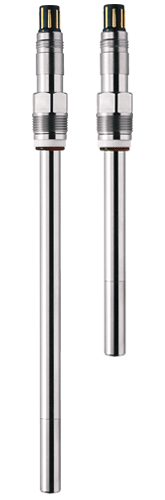
\includegraphics[scale=0.4]{editaveis/figuras/sensor_oxigenio}
	  \caption[Sensor de oxigênio dissolvido]{Sensor de oxigênio dissolvido}
	  \FloatBarrier
	  \label{sensor_oxigenio}
	 \end{figure}
	
	\begin{center}
	 \textbf{Medição de nível de fósforo total}
	\end{center}
	
	O fósforo encontrado na agua pode ter origem da dissolução doas solos e decomposição de matéria orgânica,
	do uso de fertilizantes, despejos domésticos e industriais, detergentes e excrementos animais \cite{danelon12}.
	
	Então é importante que os níveis do fósforo sejam controlados, seguindo os níveis propostos pela ANA,
	para medir-se esse parâmetro, não é possível por meio de sensores, então
	se utiliza um aparelho chamado de Fotômetro medidor de fósforo.
	  
	\begin{figure}[!h]
	  \centering
	  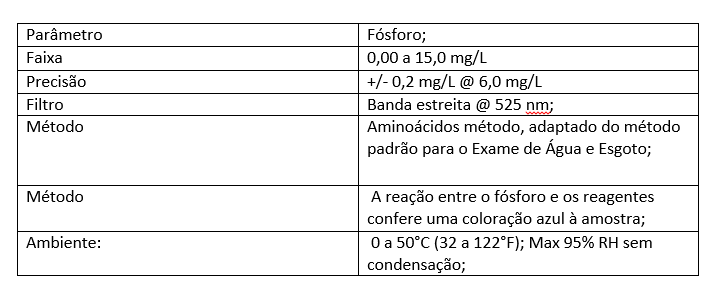
\includegraphics[scale=0.6]{editaveis/figuras/fotometro_spec}
	  \caption[Especificações de um fotômetro]{Tabela de especificações do Fotômetro (Modelo HI 96706C)}
	  \FloatBarrier
	  \label{fotometro_spec}
	 \end{figure}
	
    \item \textbf{Coliformes fecais}
    
	Coliformes totais são bactérias que não causam doenças, uma vez que habitam o intestino de animais mamíferos inclusive
	o homem. Dentre as bactérias pertencentes ao grupo coliforme totais, a mais estudada é a \textit{Escherichia Coli} (E. Coli),
	resumida como pertencente ao grupo das enterobacterias \cite{neidhardt96}.
	
	A determinação da concentração dos coliformes assume importância como parâmetro indicador da possibilidade da 
	existência de microorganismos patogênicos, responsáveis pela transmissão de doenças de veiculação hídrica, tais como
	febre tifóide, febre paratifóide, desinteria bacilar e cólera \cite{anaGovIndicadores}.
	
	A importância dos coliformes também está relacionada com a qualidade da água, uma vez que é um dos principais
	parâmetros para o cálculo do Índice de Qualidade de Água (IQA) \cite{cetesbIndiceQualidadeH2O}.
	
	A análise de coliformes deve ser realizada de acordo com as normas técnicas da CETESB que prescrevem que a análise
	deve ser realizada por meio da técnica de membrana filtrante para determinação da densidade de bactérias do grupo
	coliforme, com aplicação em: controle de qualidade de águas destinadas: ao abastecimento público (sem ou com simples
	desinfecção, ou após tratamento simplificado ou convencional); a irrigação de hortaliças e plantas; a recreação de
	contato primário (natação, esqui-aquático, mergulho); a criação natural e/ou Anais XVI Simpósio Brasileiro de
	Sensoriamento Remoto - SBSR, Foz do Iguaçu, PR, Brasil, 13 a 18 de abril de 2013, INPE 6652 intensiva (aquicultura)
	de espécies destinadas a alimentação humana; a dessedentarão de animais; ao abastecimento industrial \cite{cetesb84}.
	
	A quantidade de coliformes fecais não deve exceder um limite de 200 por 100 mililitros em 80\% ou mais de pelo menos
	5 amostras mensais colhidas em qualquer mês.
	
    \item \textbf{Anêmometro ultrasônico}
    
	Anemômetro é um equipamento que mede a velocidade e a direção dos ventos. No SI (Sistema internacional) a unidade
	utilizada para medir a velocidade do vento pode ser em m/s (metros por segundo), em km/h (quilômetros por hora) ou
	em nós \cite{almeida04}.
	
	No mercado existem vários tipos de anemômetros com diferentes exatidões, custo e métodos de medição, são alguns deles: 
	anemômetro de copo, termoelétrico e o ultrassônico.
	
	O anemômetro de copo é o mais utilizado e o mais comum no mercado \cite{cyliax06}. Ele possui vários copos ocos
	fixos em dois eixos, que se movem proporcionalmente com a velocidade do vento, que é indicada por um tacômetro. Este
	anemômetro é de baixo custo e possui precisão de mais ou menos 2\%, mas precisa ser calibrado e passar por manutenção
	periodicamente, pois tem partes móveis que se desgastam com o tempo e alteram a sua precisão.
	
	O anemômetro termoelétrico possui dois tipos o de fio e o de tubo, genericamente os dois tipos utilizam o calor dissipado
	pelos sensores do anemômetro para a medição da velocidade do vento, ou seja, o sensor é aquecido e o calor que é dissipado
	é proporcional a velocidade do vento.  O tempo de resposta do termoelétrico é maior do que o de copo, é não possui partes
	moveis, porém não é indicado para locais abertos, pois seus sensores são frágeis e os fios ou tubos acumulam impurezas,
	desse modo diminuindo sua precisão.
	
	O anemômetro ultrassônico é um tipo anemômetro que possibilita a medição da velocidade do vento , por meio da velocidade
	do som no ar.Possuisensores ultrassônicos dispostos em formato de tetraedro e em cada extremidade possui um sensor
	piezolétricos \cite{ribeiro06}, este sensor é um tipo de transdutor ultrassônicos que pode se comportar tanto
	como transdutor-transmissor quanto um transdutor-receptor, ou seja, ele pode gerar ondas ultrassônicas e também de
	recebê-las (KOYAMA,2007).
	
	O tempo que o pulso enviado por um dos sensores leva para chegar a um dos outros é medido e incrementado ou decrementado,
	dependendo da direção da velocidade do som, assim podendo obter-se a velocidade do vento nas três direções.
	
	\begin{figure}[!h]
	  \centering
	  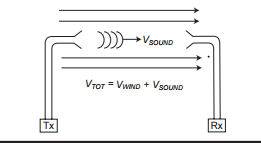
\includegraphics[scale=0.8]{editaveis/figuras/sinal_ultrasonico}
	  \caption[Soma do sinal ultrassônico e a velocidade do vento]
	    {Figura ilustrativa da soma do sinal ultrassônico e a velocidade do vento \cite{cyliax06}.}
	  \FloatBarrier
	  \label{sinal_ultrasonico}
	\end{figure}
	
	Este anemômetro é um dos mais confiáveis, não possui partes móveis, tem uma resposta rápida e com boa exatidão, não
	precisa de manutenção periódica epode ser utilizado em qualquer ambiente, sem comprometer sua precisão.
	
	Abaixo uma tabela de especificações técnicas de um anemômetro ultrassônico (Vaisala WINDCAP\textregistered WMT700):
	
	\begin{figure}[!h]
	  \centering
	  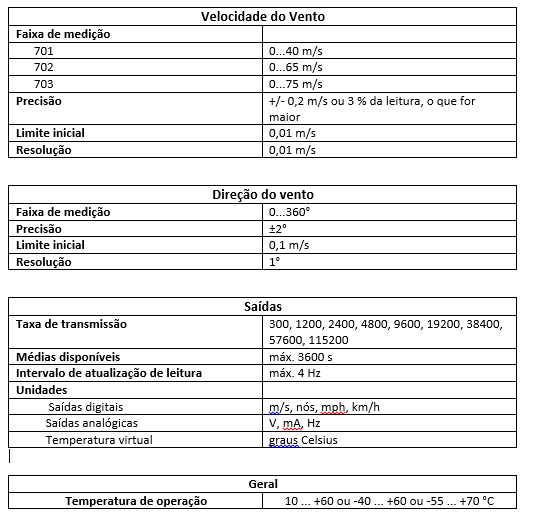
\includegraphics[scale=0.6]{editaveis/figuras/vaisala_spec}
	  \caption[Especificações técnicas do anemômetro ultrassônico Vaisala WINDCAP\textregistered WMT700]
	    {Especificações técnicas do anemômetro ultrassônico Vaisala WINDCAP\textregistered WMT700}
	  \FloatBarrier
	  \label{vaisala_spec}
	\end{figure}
	
    \item \textbf{Demanda Bioquímica de Oxigênio (DBO5,20)}
    
	Os principais métodos de determinação do DBO são o método manométrico e o método da diluição. O primeiro se baseia em
	mensurar a variação de pressão de oxigênio durante a análise, já o segundo consiste em incubação em garrafas Winkler
	(impedem que qualquer ser vivo seja capaz de realizar a fotossíntese dentro da garrafa) (UMWELT, 2015).
	
	O método da diluição envolve a medição de OD (oxigênio dissolvido) na amostra a ser analisada antes da incubação, e 
	5 dias depois da incubação. Dessa forma, a diferença entre OD final e OD inicial obtida representa a DBO5,20 (em caso 
	do ambiente de experimentação estar à 20 graus Celsius) \cite{cetesbOxigenioDissolvido}.
	
	Por outro lado, o método manométrico se baseia no consumo de oxigênio determinado pela variação de pressão. Essa diferença
	de pressão é medida com o auxílio de um sensor de pressão (piezoelétrico, por exemplo) acoplado ao topo das garrafas.
	As vantagens desse método são:
	
	\begin{itemize}
	 \item Não há necessidade de diluição da amostra;
	 \item Exibição contínua do valor de DBO durante o tempo de incubação.
	\end{itemize}
	
	Foram obtidas algumas especificações de um sensor que realizam tal tipo de medição disponível no mercado:
	
	CONTINUAR DAQUI
    
    \item \textbf{Microcontroladores}
	
	O microcontrolador é uma espécie de computador que é programado para realizar funções de acordo com o que se deseja.
	Dentro de um computador de mesa (desktop), por exemplo, existem vários microcontroladores de vários modelos e tamanhos
	que realizam diversas funções diferentes. Ou seja, são dispositivos que geralmente são embutidos no interior de um produto
	que podem controlar as funções ou ações desse produto \footnotemark. 
	\footnotetext{Disponível em: <http://tecnologia.hsw.uol.com.br/microcontroladores1.htm>}
	
	No contexto em que se encaixa este documento, os microcontroladores serão responsáveis por fazerem leituras de sinais 
	que posteriormente poderão nos informar a qualidade da água, potência em que se está sendo trabalhada a turbina,
	quantidade de água armazenada no reservatório em tempo real, a velocidade atual em que o vento atinge as turbinas,
	umidade do ar, etc. Mas para a obtenção dessas diversas informações, é necessária a utilização dos vários sensores
	citados anteriormente que vão trabalhar de modo conjunto com os microcontroladores, que formam um sistema para ler
	essas informações.
	
	Inicialmente, ao se receber a informação dentro do sistema, ela tem de ser condicionada. O condicionador mais comum é
	o amplificador. Este tem a função de amplificar sinais de baixa intensidade a fim de se aumentar sua resolução. Logo
	após isto, este sinal é enviado a um filtrador que tem por função melhorar a freqüência enviada, ou seja, ele vai
	remover sinais indesejados fazendo a freqüência permanecer no formato desejado. Dependendo de cada sinal, deverá ser
	usado um filtro diferente, pois sinais AC e DC requerem tratamentos diferenciados. Por exemplo, sensores de temperatura 
	recolhem sinais DC que geralmente são de alta freqüência, com isto, os filtradores buscam deixar esse sinal mais tênue.
	Posteriormente também se pode amplificar novamente o sinal. Essa etapa geralmente depende da ordem em que a tensão está
	chegando. Uma tensão da ordem de micro volts pode requerer ser amplificada mais uma vez para que seja sensível ao
	microcontrolador. Em sequência, o sinal deve passar por um conversor analógico digital, que tem por função passar
	informação do nosso mundo, como luz, som, para o formato digital, e então é enviado para um microcontrolador. A partir
	dessa etapa, o microcontrolador passa a informação para um transmissor que envia a informação para uma central \footnotemark.
	
	\footnotetext{Disponível em: <http://www.sabereletronica.com.br/artigos/2805-condicionamento-de-sinais-analgicos-e-sensores>}
	
	A figura ~\ref{funcionamento_microcontrolador} ilustra o funcionamento desse sistema.
	
	\begin{figure}[!h]
	  \centering
	  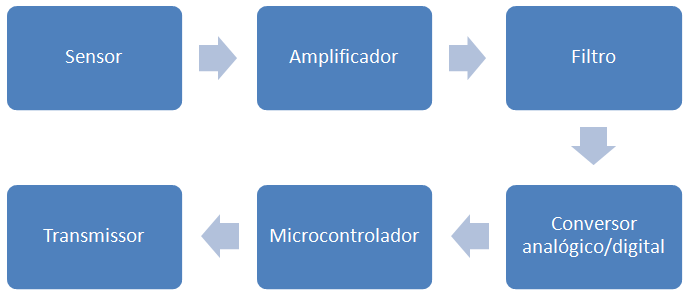
\includegraphics[scale=0.6]{editaveis/figuras/funcionamento_microcontrolador}
	  \caption[Processamento do sinal]{Processamento do sinal}
	  \FloatBarrier
	  \label{funcionamento_microcontrolador}
	\end{figure}
	
  \end{enumerate}
  
  \vfill
      
      \subsubsection{Adição de sais à água}
      
	
A água potável em sua forma pura é conhecida como água destilada. Esta água é desprovida de sais minerais ou de gases.
O consumo constante de água destilada pode ser prejudicial aos seres humano devido ao fato de a ingestão diária de sais
minerais ser complementada pelos sais presentes na água mineral. Segundo resolução da Anvisa, toda água mineral no país 
que possua como objetivo ser comercializada deve ser adicionada de sais minerais. Visando seguir esta especificação e
visando não provocar um impacto na saúde dos habitantes de Acarí optou-se por adicionar sais minerais básicos à água
retirada da umidade do ar já que a falta de sais minerais na dieta dos habitantes pode levar a doenças para os mesmos,
tais como diarreia e desidratação.

Uma das propriedades mais importantes da água é o fato de ser uma substância polar, capaz de associar-se a outras substâncias 
polares ou iônicas para formar soluções aquosas. O processo de solubilização para a planta de abastecimento de água por meio
da umidade do ar pode ser realizado por um simples processo de mistura entre os sais contidos em um reservatório e a água
provinda da turbina. Portanto, será implementado um sistema de injeção e monitoramento de sais minerais à água provinda da
turbina que contará com processos mecânicos e digitais.

\begin{center}
\textbf{Mecanismos para a adição dos sais minerais}
\end{center}

  Para a adição de sais minerais na água, será implementado um mecanismo baseado em equipamentos já existentes, que injetarão
  sais minerais na água provinda da turbina. Para a realização de um processo automático de inserção de sais, será necessária 
  a utilização de um dosador automático, que varia a dosagem de uma substância de acordo com as concentrações da mesma na mistura 
  que será constantemente verificada. Existem equipamentos como o Dosimat 865, da empresa Metrohm, que possui o modo de operação
  CNT D: ao ser inserida a concentração final que se deseja de uma substância, o dosador é capaz de determinar o volume de água
  a ser adicionado para que a concentração desejada seja mantida.
  
  \begin{figure}[!htbp]
    \centering
    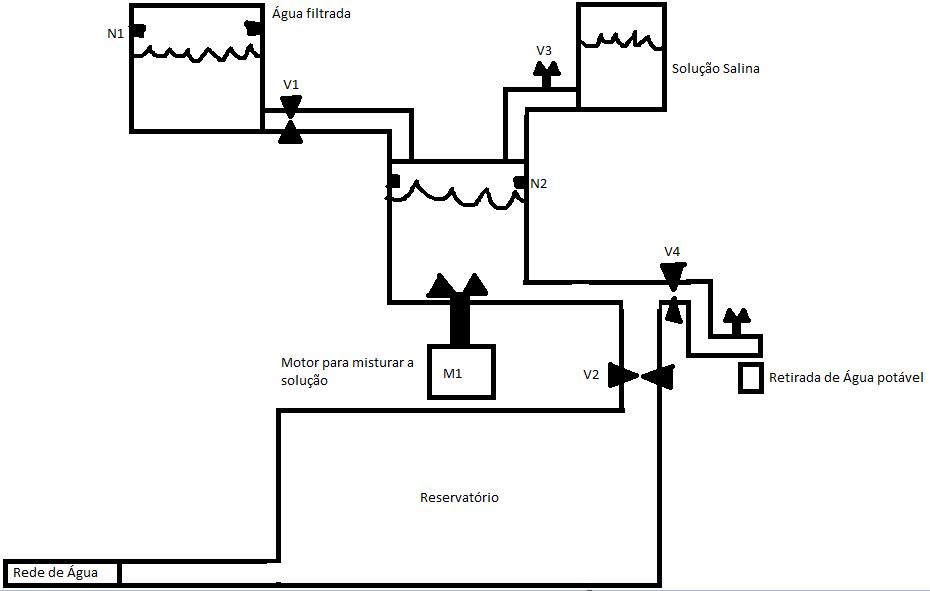
\includegraphics[scale=0.6]{editaveis/figuras/funcionamento_adicao_sais}
    \caption[Esquemático de funcionamento do controle de adição de sais]{Esquemático de funcionamento do controle de adição de sais.}
    \label{funcionamento_adicao_sais}
  \end{figure}
  \FloatBarrier
    
\begin{center}
\textbf{Funcionamento básico do sistema}
\end{center}

  \begin{itemize}
   
   \item O \textbf{sistema de controle} terá a função de enviar comandos e desta forma realizar o controle mecânico da comporta 
   que abre e fecha o tanque de armazenamento da água retirada da umidade do ar. Este sistema terá acesso direto ao aparelho
   dosador e ao sistema de sensoriamento, pois, por meio dele terá acesso às concentrações dos sais no tanque de adição. 
   Quando as concentrações de sais no tanque de adição estiverem altas, a comporta se abrirá e mais água será adicionada à 
   mistura. Por outro lado, quando as concentrações de sais estiverem baixas no tanque de adição, os comandos serão dados
   para que a comporta seja fechada. Este processo ocorrerá até que as concentrações ideais dos sais sejam atingidas.
   
   \item A \textbf{válvula de retenção} será utilizada para que a água flua apenas em um sentido, que no caso do esquemático 
   seria da esquerda para a direita. Isto impedirá que a água já adicionada de sais retorne ao tanque da água retirada da
   umidade do ar.
   
   \item O \textbf{tanque para adição de sais} será o reservatório que conterá a água adicionada de sais. Neste tanque, além
   de ocorrer a adição de sais, ocorrerá também o processo de mistura para que a solubilização dos sais na água aconteça de
   forma uniforme.
   
   \item Para o \textbf{sensoriamento} do tanque de adição de sais poderá ser utilizado um sensor de condutividade.
   Este sensor possui grande aplicabilidade a este sistema de sensoriamento, pois “A água tem um forte poder de dissociação,
   pode separar o material dissolvido em íons carregados eletronicamente. Como consequência, o material dissolvido aumenta
   bastante a condutividade da água” \cite{abilio05}.
   
  \end{itemize}
  
\begin{center}
\textbf{Misturador e dosador automático}
\end{center}

Este sistema é utilizado por empresas brasileiras para a adição de sais na água in-natura através de processos
físicos com o objetivo de produzir água tratada que é devidamente envasada e posteriormente vendida.

O princípio básico do misturador é uma máquina que provoca intensa agitação na água, dissolvendo os sais minerais. Um 
exemplo de misturador e dosador automático pode ser visto na imagem abaixo. Este equipamento é utilizado pela empresa
Amazônia- Água adicionada de sais, que produz água adicionada de sais no estado do Pará.

\begin{figure}[!htbp]
  \centering
  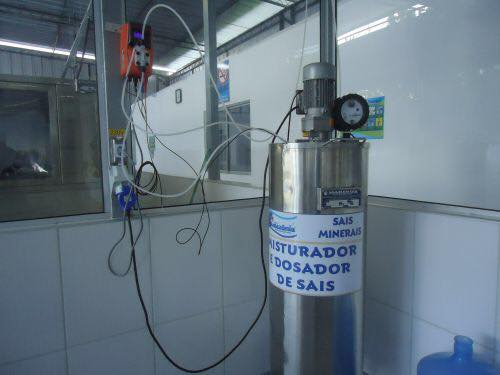
\includegraphics[scale=0.6]{editaveis/figuras/dosador_sais}
  \caption[Misturador e dosador de sais]{Misturador e dosador de sais. \footnotemark}
  \label{funcionamento_adicao_sais}
\end{figure}
\footnotetext{http://www.aguaamazonia.com/?page\_id=111}.
\FloatBarrier


\begin{center}
\textbf{Filtro adicionador de sais}
\end{center}

Existem no mercado filtros patentiados que realizam o processo de adição de sais, um bom exemplo é o ALKA WATER Biocal Ceramic 
Filter, que segundo a empresa Alka Water é um filtro que adiciona íons de cálcio, magnésio, sódio e potássio, além de ser 
aprovado pela FDA (\textit{Food and Drug Administration}).

O processo é realizado de forma passiva, necessitando apenas que a água passe pelo filtro e posteriormente seja misturada para
que a adição de sais seja realizada de maneira adequada. Um esquemático simplificado deste processo pode ser observado na imagem abaixo.

\begin{figure}[!htbp]
  \centering
  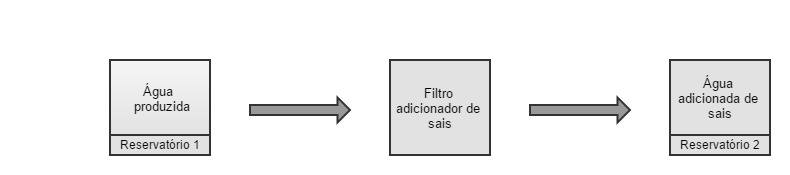
\includegraphics[scale=0.6]{editaveis/figuras/esquema_filtro_adicionador_sais}
  \caption[Esquemático do filtro adicionador de sais]{Esquemático do filtro adicionador de sais.}
  \label{esquema_filtro_adicionador_sais}
\end{figure}
\FloatBarrier



       
    \pagebreak  
    \subsection{Sistema de Gestão da Informação do monitoramento da qualidade da água}
	
	
\subsubsection{Softwares de monitoramento de água}

  	Este tópico baseia-se no estudo de softwares existentes no mercado que possuem o intuito de testar a qualidade da água,
	para assim dar a segurança nescessária de qualidade ao consumo humano, de acordo a constituição vigente, e as normas
	de qualidade de saúde determinadas pela Agência Nacional de Águas (\citeauthor{anaGov}).
	
	Estes softwares poderão ser aplicados no sistema de armazenamento da água coletada através do ar, uma vez que as
	partículas de água podem conter substâncias químicas, o que torna a água inapropriada ao consumo. Devem ser utilizados
	com o auxilio de sensores para coleta dos dados. \\

% \begin{center}
\noindent
\textbf{Water Quality Analyser} (Fonte: \citeauthor{eWater})
% \end{center}	

	Com uma interface de usuário simples e direta possuindo foco na visualização de entradas e saídas de dados, este
	software ajuda a identificar a qualidade de água e simplificar o caminho para uma breve avaliação, através de
	ferramentas, que comparam a qualidade da água com os termos legais previamente definidos.
	
	Utiliza um gerenciamento de dados, para validação, vizualização e apresentação de relatórios, além de fornecer
	estatísticas de mudanças e aleatoriedade na qualidade da aguá, além de outros dados temporais.
	
	Este software foi desenvolvido pela colaboração, entre a empresa eWater CRC e o Departamento de Meio Ambiente
	e Gestão de Recursos de Queensland (QDERM), na Australia.
	
	A ferramenta é paga custando \$299 dollares, equivalente á R\$ 892,89 reais (cotação de 20/04/2015 - preço do
	dollar 2,98) pelo licenciamento de um ano, possuindo a possibilidade de teste gratuito pelo período de 30 dias.

	
\textbf{Prós:}
	
\begin{itemize}
  \item Muitas ferramentas;
  \item Interface simples;
  \item Recomendado para utilização em escala industrial;
 \end{itemize}
 
\textbf{Contras:}
	
\begin{itemize}
  \item Disponível apenas em inglês;
  \item Ferramenta paga;\\
 \end{itemize}

 
% \begin{center}
\noindent
\textbf{Logger Pro} (Fonte: \citeauthor{loggerPro})
% \end{center}	

	Utiliza coleta de dados em tempo real, suportando mais de 80 sensores e dispositivos diferentes, apresenta os dados
	em interface aceitando os sistemas operacionais Windows ou MAC.
	
	Custa \$339, equivalente à R\$1.012,34 (cotação de 20/04/2015 - preço do dollar 2,98). Possuindo uma versão Lite,
	gratuita e com menos funcionalidades.
	
\textbf{Prós:}
	
\begin{itemize}
  \item Multiuso, com muitas ferramentas;
  \item Coleta em tempo real;
  \item Captura vídeos;
  \item Desenha previsões utilizando gráficos de dados coletados anteriormente;
  \item Realiza análise estática dos dados;
  \item Possui gráficos avançados com ajuste de função;
  \item Transmição sem fio para dispositivos móveis;
 \end{itemize}
 
\textbf{Contras:}
	
\begin{itemize}
  \item Preço dos equipamentos;
  \item Feito para nível estudantil;\\
 \end{itemize}
 

% \begin{center}
\noindent
\textbf{AquaChem} (Fonte: \citeauthor{aquaChem})
% \end{center}	

	Ferramenta para análise cobrindo uma ampla gama de funções e cálculos utilizados para análise, interpretação 
	e comparação de dados da qualidade da aguá. Possuindo estatísticas e funções mais complexas, como matrizes de
	correlação e cálculos análiticos.
	
	Possui preço em dólares variando entre 1.355,75(R\$ 4.048,61) até 2.390,50 (R\$ 7.138,63).
	
\textbf{Prós:}
	
\begin{itemize}
  \item Cálculos geoquímicos;
  \item Análise simples e fácil de dados de qualidade da água;
  \item Cálculos estatísticos;
  \item Criado para escala comercial;
\end{itemize}
 
\textbf{Contras:}
	
\begin{itemize}
  \item Alto custo;
\end{itemize}  
  
% \subsubsection{Integração com o sistema eletrônico}
% 
%   Para analisar a qualidade da água são necessários sensores, os dados obtidos por esses sensores são transmitidos para
unidades com capacidade de processamento, para computadores. Os dados obtidos por esses sensores individualmente devem
ser analisados via software. Para efetuar a análise da qualidade da água, é necessária uma análise dos dados obtidos
pelo conjunto desses sensores, pois cada um indica uma ou algumas características específicas da água e não a qualidade
como um todo.

O software a ser utilizado depende basicamente do circuito eletrônico escolhido, tanto do computador, como dos tipos
e especificações dos sensores. Para medir a qualidade da água serão utilizados sensores capazes de avaliar basicamente
o nível de PH, oxigênio dissolvido, temperatura, íons dissolvidos, turbidez, resíduo total da água.

No software será definido o intervalo em que cada um dos indicadores de qualidade é aceitável para consumo humano de
acordo com a análise feita pelo grupo.  Em algumas situações, não seguiremos estritamente os padrões estipulados pelas 
agências reguladoras, desde que a escolha esteja dendro do estipulado por elas e traga algum benefício aos usuários. 
Por exemplo, o valor ideal de PH da água para consumo humano é de 6 a 9, porém a Agência Nacional de Vigilância Sanitária (ANVISA)
não estabelece nenhuma resolução indicando um valor mínimo para o pH.

Outro aspecto importante do software é que ele impeça a passagem da água, caso ela esteja fora dos padrões de qualidade
estipulados, até que o tratamento ocorra e seja finalizado. Para que isso ocorra,  o software fará uma uma comparação
entre cada um dos índices com os valores adequados e, caso a água não esteja dentro do padrão, o hardware enviará um 
sinal elétrico, comandando um mecanismo eletromecânico capaz de bloquear a passagem de água.

Além da análise da qualidade da água, será necessário sensores para analisar o nível da água tanto no reservatório
de distribuição de água, como no reservatório de armazenamento de água para tratamento. Os dados relacionados ao nível 
e qualidade da água serão transmitidos para um outro sistema que possibilita uma interação com o usuário, composto por
um software diferente.

Pretende-se utilizar a linguagem C/C++ para a elaboração do software relacionado ao controle da água. Estas linguagens
pode ser compiladas e utilizadas para uma grande parte dos sistemas embarcados. Para o desenvolvimento, será feito uma
análise mais profunda do problema, serão levantados todos os requisitos funcionais e não funcionais do software, a 
arquitetura, além disso, serão feitos testes ao longo do processo de desenvolvimento.

Além desse software, será necessário o desenvolvimento de outros, que estão mais relacionados à interação com o ser
humano, apresentando para o usuário os índices de qualidade da água. Esses softwares serão executados por hardwares
mais potentes e,  portanto, não haverá tantas limitações de processamento e memória. Dessa forma, não será necessário
fazer uma análise profunda da interação entre a eletrônica e o software, embora seja necessário uma análise dos 
sistemas operacionais, linguagens que possam ser interpretadas ou compiladas para ele.
  
\subsubsection{Interface homem-máquina}

    
  O presente trabalho não irá fornecer um sistema completo com todas as funcionalidades implementadas,
  apenas um protótipo da interface com o usuário. Para tal, é necessário o entendimento de alguns conceitos de
  Interação Humano-Computador.\\
  
  \noindent
  \textbf{Usabilidade}
  
  No processo de produção de software, uma parte importante é a produção de protótipos. Esses protótipos sevem
  como base para a validação de requisitos, além de serem usados para a avaliação de usabilidade do software.
  Sendo assim, os softwares que serão desenvolvidos devem seguir os seis princípios de usabilidade, segundo \cite{preece02}, que são:
 
 \begin{itemize}
  \item Eficácia: O software deverá fazer bem o que lhe foi destinado a fazer.
  \item Eficiência: O software deverá fazer suas funções de modo rápido e fácil.
  \item Segurança: O software deverá prevenir o usuários de cometer erros que prejudiquem a realização do que o usuário deseja.
  \item Utilidade: O software deverá ser útil.
  \item Capacidade de aprendizagem: O software deverá ser fácil de ser utilizado.
  \item Capacidade de memorização: Após a primeira vez de uso, o usuário deverá ser capaz de utilizar o software novamente com mais facilidade do que na primeira vez.
 \end{itemize}
 
	Para a construção dos protótipos, serão utilizados ferramentas de mockup, abaixo estão listadas algumas no mercado:
     
\begin{center}
\textbf{Balsamiq}
\end{center}	

	A ferramenta Balsamiq Mockup permite a criação de protótipos e modelos de baixa e alta fidelidade,
	para sistemas desktop, web ou mobile.
	
\textbf{Prós:}
	
\begin{itemize}
  \item Interface Intuitiva;
  \item Possui versão para desktop;
  \item Versão trial de 30 dias;
  \item Preço baixo para a licença;
 \end{itemize}
 
\textbf{Contras:}
	
\begin{itemize}
  \item Não oferece equipe de suporte;
 \end{itemize}
     
     
     
\begin{center}
\textbf{Mockingbird}
\end{center}	

	É uma ferramenta online que permite a criação e compartilhamento de protótipos.
	
\textbf{Prós:}
	
\begin{itemize}
  \item Interface Intuitiva;
  \item Possui equipe de suporte;
  \item Ferramenta gratuita;
 \end{itemize}
 
\textbf{Contras:}
	
\begin{itemize}
  \item Não poussi aplicação offline;
 \end{itemize}
      
     
     
\begin{center}
\textbf{MockFlow}
\end{center}	

	Conjunto de wireframing profissional para projetar interfaces.
	
\textbf{Prós:}
	
\begin{itemize}
  \item Interface Intuitiva;
  \item Versão online ou desktop;
  \item Ferramentas para trabalhar em equipe;
\end{itemize}
 
\textbf{Contras:}
	
\begin{itemize}
  \item Versão free limitada a 4 páginas;
  \item Não possui a opção de pagamento mensal;
  \item Baseado em Flash;
\end{itemize}
      
  \section{Requisitos do sistema}
  
      O projeto possui 4 frentes de requisitos. São elas:
      
      \begin{itemize}
	\item Requisitos do projeto estrutural mecânico do sistema de captação da água e do transporte para a central de armazenamento;\\
	 
	 \textbf{Requisitos funcionais}
	  \begin{itemize}
	   \item Retirar água da umidade do ar;
	   \item Bombear água para o reservatório;
	  \end{itemize}
	  
	  \textbf{Requisitos não-funcionais}
	  \begin{itemize}
	   \item O sistema deve atender a uma demanda de água diária;
	   \item O sistema deve bombear toda água por dia produzida pro reservatório; 
       \item O sistema deve ser composto por materiais resistentes à água;
       \item O sistema deve possuir um reservatório de capacidade de até 3 dias de água;
       \item O sistema deve operar com incidências de ventos de 7 a 50 m/s, umidade a partir de 40\% e 	temperatura à partir de $26\,^{\circ}\mathrm{C}$\cite{eole}
       \item O sistema deve aproveitar o relevo da região para o transporte da água;

	  \end{itemize}
	  
	\item Requisitos do projeto dos circuitos eletrônicos que irão compor o sistema de monitoramento e controle da qualidade da água.\\
	 
	 \textbf{Requisitos funcionais}
	  \begin{itemize}
	   \item Atuar como um sistema de controle dos elementos do sistema de modo a produzir a saída desejada (manter a água própria para o consumo humano);
	   \item Obter informações climáticas da região;
	   \item Obter dados do estado reservatório;
	   \item Ler parâmetros que definem a qualidade da água;
	   \item Efetuar conversão analógica/digital dos sinais filtrados;
	   \item Processar o sinal convertido de modo que os dados possam ser transmitidos ao usuário;
	   \item Exibir dados obtidos ao usuário;
	  \end{itemize}
	  
	  \textbf{Requisitos não-funcionais}
	  \begin{itemize}
	   \item Utilizar sensores para obtenção dos dados;
	   \item Exibir dados dos sensores ao usuário em tempo real;
	   \item Utilizar filtros analógicos para retirar eventuais ruídos que a saída do sensor possa gerar;
	  \end{itemize}
	  
	\item Requisitos do projeto do sistema de Gestão da Informação do monitoramento da qualidade da água;\\
	 
	 \textbf{Requisitos funcionais}
	  \begin{itemize}
	   \item Apenas o moderador poderá, modificar os dados.
	   \item O sistema registrará os dados de qualidade da agua.
	   \item O sistema deve emitir um alerta caso um parâmetro de qualidade não esteja aceitável.
	   \item O sistema deve permitir consultas dos dados armazenados de datas anteriores.
	   \item O sistema deve possuir uma interface pare exibir os dados.
	   \item O sistema deve possuir uma página de \textit{login} antes de entrar no sistema.
	   \item O sistema deve possuir um mecanismo de impressão dos dados.
	   \item O sistema possuirá um mecanismo para exportar os dados.
	  \end{itemize}
	  
	  \textbf{Requisitos não-funcionais}
	  \begin{itemize}
	   \item O sistema deve ser fácil de usar, evitando excesso de digitação, de modo a dar agilidade ao processo.
	   \item O sistema deve possuir uma interface simples.
	   \item O sistema deve funcionar no sistema operacional Windows.
	   \item O sitema deve monitorar as amostras de água a cada 30 mimutos.
	  \end{itemize}
	
	\item Requisitos do projeto da matriz energética que dará o suporte para o sistema de captação de água e o sistema de monitoramento da qualidade da água;\\
	
	 \textbf{Requisitos funcionais}
	  \begin{itemize}
	   \item Produzir energia elétrica através da energia eólica;
	   \item Converter energia cinética em energia elétrica;
	   \item Armazenar a energia elétrica gerada;
	   \item Fornecer energia para os componentes eletrônicos, de controle e monitoramento do produto final;
	   \item Fornecer energia para o bombeamento mecânico de água.
	  \end{itemize}
	  
	  \textbf{Requisitos não-funcionais}
	  \begin{itemize}
	   \item Utilizar uma fonte renovável de energia;
	   \item Ser autossuficiente no quesito energia gerada-consumida;
	   \item Possuir eficiência energética aceitável;
	   \item Ser estável energeticamente;
	  \end{itemize}
	  
      \end{itemize}
    
    
    
    